%
%
%

\newpage

\section{Proofs}
\begin{proof}[Proof of Lemma \ref{lemma:weights-est}]
First, we express the weights $w(y)$ as the conditional expectation as follows:
\begin{align*}
    w(y) &= \frac{\ptar(y)}{\pbeh(y)} \\
    &= \int_{\Xspace, \Aspace} \frac{\ptar(x,a,y)}{\pbeh(y)}\,\mathrm{d}a\, \mathrm{d}x\\
    &= \int_{\Xspace, \Aspace} \frac{\ptar(x,a,y)}{\pbeh(y)}\,\frac{\pbeh(x, a\mid y)}{\pbeh(x, a\mid y)}\,\mathrm{d}a\, \mathrm{d}x\\
    &= \int_{\Xspace, \Aspace} \frac{\ptar(x,a,y)}{\pbeh(x, a, y)}\,\pbeh(x, a\mid y)\,\mathrm{d}a\, \mathrm{d}x\\
    &= \int_{\Xspace, \Aspace} \rho(a, x)\,\pbeh(x, a\mid y)\,\mathrm{d}a\, \mathrm{d}x\\
    &= \Ebeh[\rho(A, X)\mid Y=y],
\end{align*}
where $\rho(a, x) = \frac{\ptar(x, a, y)}{\pbeh(x, a, y)} = \frac{\tar(a\mid x)}{\beh(a\mid x)}$.
Since conditional expectations can be defined as the solution of regression problem, the result follows. 
\end{proof}

\begin{proof}[Proof of Proposition \ref{tv_prop}] We have
\begin{align*}
    \textup{D}_f\left(\ptar(x,a,y)\,||\, \pbeh(x,a,y)\right) &= \Ebeh\left[ f\left( \frac{\ptar(X,A,Y)}{\pbeh(X,A,Y)}\right) \right]\\
    &= \Ebeh\left[ f\left( \frac{\tar(A\mid X)}{\beh(A\mid X)}\right) \right]\\
    &= \Ebeh\left[\Ebeh\left[ f\left( \frac{\tar(A\mid X)}{\beh(A\mid X)}\right) \Bigg| Y \right]\right]\\
    &\geq \Ebeh\left[ f\left( \Ebeh\left[\frac{\tar(A\mid X)}{\beh(A\mid X)}\Bigg| Y \right]\right) \right]\quad\text{(Jensen's inequality)}\\
    &= \Ebeh\left[ f\left( \frac{\ptar(Y)}{\pbeh(Y)} \right) \right]\\
    &= \textup{D}_f\left(\ptar(y)\,||\, \pbeh(y)\right).
\end{align*}
\end{proof}

\begin{proof}[Proof of Proposition \ref{prop:var_mr}]
Since $\Ebeh[\thetaipw] = \Ebeh[\thetamr] = \Etar[Y]$, we have that,  
\begin{align*}
    \Vbeh[\thetaipw] - \Vbeh[\thetamr] &= \Ebeh[\thetaipw]^2 - \Ebeh[\thetamr]^2 \\
    &= \frac{1}{n} \left(\Ebeh\left[\rho(A, X)^2\, Y^2 \right] - \Ebeh\left[w(Y)^2\, Y^2 \right] \right)\\
    &= \frac{1}{n} \left(\Ebeh\left[\Ebeh[\rho(A, X)^2\mid Y]\, Y^2 \right] - \Ebeh\left[w(Y)^2\, Y^2 \right] \right)\\
    &= \frac{1}{n} \left(\Ebeh\left[\Ebeh[\rho(A, X)^2\mid Y]\, Y^2 \right] - \Ebeh\left[\Ebeh[\rho(A, X)\mid Y]^2\, Y^2 \right] \right)\\
    &= \frac{1}{n} \Ebeh \left[ \Vbeh\left[ \rho(A, X) \mid Y \right]\, Y^2 \right].
\end{align*}
In the second last step above, we use the fact that $w(y) = \Ebeh[\rho(A, X)\mid Y=y]$. 
\end{proof}

\begin{proof}[Proof of Proposition \ref{prop:var_dr}]
Let $\hat{\mu}(a, x) \approx \E[Y\mid X=x, A=a]$ denote the outcome model in DR estimator. Then, using multiple applications of the law of total variance we get that
\begin{align*}
    n\, \Vbeh[\thetadr] &= \Vbeh\left[\rho(A, X)\,(Y - \hat{\mu}(A, X)) + \sum_{a'\in \Aspace} \hat{\mu}(a', X)\,\tar(a'\mid X)\right]\\
    &= \Vbeh\left[\rho(A, X)\,(Y - \hat{\mu}(A, X)) + \Etar[\hat{\mu}(A, X)\mid X]\right]\\
    &= \Ebeh[\Vbeh[\rho(A, X)\,(Y - \hat{\mu}(A, X)) + \Etar[\hat{\mu}(A, X)\mid X]\mid X, A]]\\
    &\quad+ \Vbeh[\Ebeh[\rho(A, X)\,(Y - \hat{\mu}(A, X)) + \Etar[\hat{\mu}(A, X)\mid X]\mid X, A]]\\
    &= \Ebeh[\rho(A, X)^2 \var[Y\mid X, A]] \\
    &\quad+ \Vbeh[\Ebeh[\rho(A, X)\,(Y - \hat{\mu}(A, X)) + \Ebeh[\rho(A, X)\,\hat{\mu}(A, X)\mid X]\mid X, A]]\\
    &= \Ebeh[\rho(A, X)^2 \var[Y\mid X, A]] \\
    &\quad+ \Vbeh[\rho(A, X)\,(\mu(A, X) - \hat{\mu}(A, X)) + \Ebeh[\rho(A, X)\,\hat{\mu}(A, X)\mid X]]\\
    &= \Ebeh[\rho(A, X)^2 \var[Y\mid X, A]] \\
    &\quad+ \Vbeh[\Ebeh[\rho(A, X)\,(\mu(A, X) - \hat{\mu}(A, X)) + \Ebeh[\rho(A, X)\,\hat{\mu}(A, X)\mid X]\mid X]] \\
    &\quad+ \Ebeh[\Vbeh[\rho(A, X)\,(\mu(A, X) - \hat{\mu}(A, X)) + \Ebeh[\rho(A, X)\,\hat{\mu}(A, X)\mid X]\mid X]]\\
    &= \Ebeh[\rho(A, X)^2 \var[Y\mid X, A]]+ \Vbeh[\Ebeh[\rho(A, X)\,\mu(A, X)\mid X]] \\
    &\quad+ \Ebeh[\Vbeh[\rho(A, X)\,(\mu(A, X) - \hat{\mu}(A, X))\mid X]]\\
    &\geq \Ebeh[\rho(A, X)^2 \var[Y\mid X, A]] + \Vbeh[\Ebeh[\rho(A, X)\,\mu(A, X)\mid X]].
\end{align*}
Using this, we get that
\begin{align*}
    &n (\Vbeh[\thetadr] - \Vbeh[\thetamr]) \\
    &\quad\geq \Ebeh[\rho(A, X)^2 \var[Y\mid X, A]] +  \Vbeh \left[\Ebeh[\rho(A, X) \,\mu(A, X)\mid X]\right] - \Vbeh[w(Y)\,Y].
\end{align*}
Again, using the law of total variance,
\begin{align*}
    \Vbeh[\rho(A, X)\,Y] &= \Ebeh[\Vbeh[\rho(A, X)\,Y \mid X, A]] + \Vbeh[\Ebeh[\rho(A, X)\,Y\mid X, A]]\\
    &= \Ebeh[\rho(A, X)^2\var[Y \mid X, A]] + \Vbeh[ \rho(A, X)\,\mu(A, X)]\\
    &= \Ebeh[\rho(A, X)^2\var[Y \mid X, A]] + \Vbeh \left[\Ebeh[\rho(A, X) \,\mu(A, X)\mid X]\right] \\
    &\quad+ \Ebeh \left[\Vbeh[\rho(A, X) \,\mu(A, X)\mid X]\right].
\end{align*}
Rearranging and substituting back into the expression earlier, we get that
\begin{align*}
    &n (\Vbeh[\thetadr] - \Vbeh[\thetamr]) \\
    &\quad\geq \Vbeh[\rho(A, X)\,Y] - \Ebeh \left[\Vbeh[\rho(A, X) \,\mu(A, X)\mid X]\right] - \Vbeh[w(Y)\,Y].
\end{align*}
Now, from Proposition \ref{prop:var_mr} we know that \begin{align*}
    n (\Vbeh[\thetaipw] - \Vbeh[\thetamr]) = \Vbeh[\rho(A, X)\,Y] - \Vbeh[w(Y)\,Y] = \Ebeh \left[ \Vbeh\left[ \rho(A, X) \mid Y \right]\, Y^2 \right].
\end{align*}
Therefore, 
\begin{align*}
    &n (\Vbeh[\thetadr] - \Vbeh[\thetamr]) \\
    &\quad\geq \Ebeh \left[ \Vbeh\left[ \rho(A, X) \mid Y \right]\, Y^2 \right] - \Ebeh \left[\Vbeh[\rho(A, X) \,\mu(A, X)\mid X]\right]\\
    &\quad= \Ebeh \left[\Vbeh\left[ \rho(A, X)\,Y \mid Y \right] - \Vbeh[\rho(A, X) \,\mu(A, X)\mid X] \right].
\end{align*}
\end{proof}

%
%
%
%
%
%
%
%
%
%
%
%
%
%
%
%
%
%
%
%
%
%
%
%
%
%
%
%
%
%
%
%
%
%

\begin{comment}
    

\begin{proof}[Proof of Proposition \ref{prop:mips_var_reduction}]
The following proof, which is included for completeness, is a straightforward extension of \cite[Theorem 3.6]{saito2022off}. 
\begin{align*}
    &n (\Vbeh[\thetaipw] - \Vbeh[\hat{\theta}_{\textup{MIPS}}])\\
    &\quad= \Vbeh\left[\frac{\tar(A|X)}{\beh(A|X)}\,Y\right] - \Vbeh\left[\frac{\ptar(R)}{\pbeh(R)}\,Y \right]\\
     &\quad= \Vbeh\left[\Ebeh\left[\frac{\tar(A|X)}{\beh(A|X)}\,Y \Bigg| R\right]\right] + \Ebeh\left[ \Vbeh\left[\frac{\tar(A|X)}{\beh(A|X)}\,Y\Bigg| R \right]\right] - \Vbeh\left[\Ebeh\left[ \frac{\ptar(R)}{\pbeh(R)}\,Y \Bigg| R\right]\right]\\
     &\qquad- \Ebeh\left[\Vbeh\left[ \frac{\ptar(R)}{\pbeh(R)}\,Y \Bigg| R\right]\right]
\end{align*}
Now using the conditional independence Assumption \ref{assum:indep-general}, the first term on the RHS above becomes,
\begin{align*}
    \Vbeh\left[\Ebeh\left[\frac{\tar(A|X)}{\beh(A|X)}\,Y \Bigg| R\right]\right] &= \Vbeh\left[\Ebeh\left[\frac{\tar(A|X)}{\beh(A|X)}\Bigg| R\right]\,\Ebeh\left[Y | R\right]\right]\\
    &= \Vbeh\left[\frac{\ptar(R)}{\pbeh(R)}\,\Ebeh\left[Y | R\right]\right],
\end{align*}
where in the last step above we use the fact that
\begin{align*}
    \Ebeh\left[\frac{\tar(A|X)}{\beh(A|X)}\Bigg| R\right] = \frac{\ptar(R)}{\pbeh(R)}.
\end{align*}
Putting this together, we get that
\begin{align}
    &n (\Vbeh[\thetaipw] - \Vbeh[\hat{\theta}_{\textup{MIPS}}]) \nonumber\\ 
    &\quad= \Ebeh\left[ \Vbeh\left[\frac{\tar(A|X)}{\beh(A|X)}\,Y\Bigg| R \right]\right] - \Ebeh\left[\Vbeh\left[ \frac{\ptar(R)}{\pbeh(R)}\,Y \Bigg| R\right]\right]. \label{eq:variance-difference}
\end{align}
Since we have that 
\begin{align*}
    \Ebeh\left[\frac{\tar(A|X)}{\beh(A|X)}\,Y\Bigg| R \right] = \Ebeh\left[\frac{\tar(A|X)}{\beh(A|X)}\Bigg| R \right]\,\Ebeh\left[Y| R \right] = \frac{\ptar(R)}{\pbeh(R)}\,\Ebeh\left[Y| R \right],
\end{align*}
Eq. \eqref{eq:variance-difference} becomes,
\begin{align*}
    &\Ebeh\left[ \Vbeh\left[\frac{\tar(A|X)}{\beh(A|X)}\,Y\Bigg| R \right]\right] - \Ebeh\left[\Vbeh\left[ \frac{\ptar(R)}{\pbeh(R)}\,Y \Bigg| R\right]\right] \\
    &\quad= \Ebeh\left[ \Ebeh\left[ \left(\frac{\tar(A|X)}{\beh(A|X)}\,Y \right)^2\Bigg| R  \right] - \Ebeh\left[ \left(\frac{\ptar(R)}{\pbeh(R)}\,Y \right)^2\Bigg| R \right] \right]\\
    &\quad= \Ebeh\left[ \Ebeh\left[ \left(\frac{\tar(A|X)}{\beh(A|X)} \right)^2 \Bigg| R  \right] \, \Ebeh\left[Y^2 | R  \right] - \left(\frac{\ptar(R)}{\pbeh(R)}\right)^2\,\Ebeh\left[Y^2 | R \right] \right]\\
    &\quad= \Ebeh\left[\Ebeh\left[Y^2 | R \right]\, \left( \Ebeh\left[ \left(\frac{\tar(A|X)}{\beh(A|X)} \right)^2 \Bigg| R  \right] - \left(\Ebeh\left[ \frac{\tar(A|X)}{\beh(A|X)} \Bigg| R  \right]\right)^2\, \right) \right]\\
    &\quad=\Ebeh\left[\Ebeh\left[Y^2 | R \right]\, \Vbeh\left[\frac{\tar(A|X)}{\beh(A|X)} \Bigg| R \right]\right].
\end{align*}
\end{proof}
\end{comment}
\begin{comment}

\begin{proof}[Proof of Proposition \ref{prop:bias-and-var}]
\begin{align*}
    \textup{Bias}(\thetaipw) &= \Ebeh[\hat{\rho}(A, X)\, Y] - \Etar[Y] \\
    &= \Ebeh\left[\Ebeh[\hat{\rho}(A, X)\mid Y]\,Y \right] - \Etar[Y]  \\
    &= \Ebeh[\hat{w}(Y)\, Y] - \Etar[Y] \\
    &= \textup{Bias}(\thetadr)
\end{align*}
Next, we prove the variance result.
As shown above, $\Ebeh[\thetaipw] = \Ebeh[\thetamr]$. Therefore, we have that,  
\begin{align*}
    \Vbeh[\thetaipw] - \Vbeh[\thetamr] &= \Ebeh[\thetaipw]^2 - \Ebeh[\thetamr]^2 \\
    &= \frac{1}{n} \left(\Ebeh\left[\hat{\rho}(A, X)^2\, Y^2 \right] - \Ebeh\left[\hat{w}(Y)^2\, Y^2 \right] \right)\\
    &= \frac{1}{n} \left(\E_{Y\sim\pbeh(Y)}\left[\Ebeh[\hat{\rho}(A, X)^2\mid Y]\, Y^2 \right] - \Ebeh\left[\hat{w}(Y)^2\, Y^2 \right] \right)\\
    &= \frac{1}{n} \left(\E_{Y\sim\pbeh(Y)}\left[\Ebeh[\hat{\rho}(A, X)^2\mid Y]\, Y^2 \right] - \E_{Y\sim\pbeh(Y)}\left[\Ebeh[\hat{\rho}(A, X)\mid Y]^2\, Y^2 \right] \right)\\
    &= \frac{1}{n} \E_{Y\sim \pbeh(Y)} \left[ \Vbeh\left[ \hat{\rho}(A, X) \mid Y \right]\, Y^2 \right].
\end{align*}
Where, in the second last step above we use the fact that almost surely, $\hat{w}(Y) = \Ebeh[\hat{\rho}(A, X)\mid Y]$.
\end{proof}
\end{comment}


%
%

%
%
%
%
%
%
%
%
%
%
%
%
%
%
%
%
%
%
%
%
%
%
%
%
%
%
%
%
%
%
%
%
%
%
%
%
%
%
%
%
%
%
%
%
%
%
%
%
%

%
%
%
%
%
%

\begin{proof}[Proof of Theorem \ref{prop:mips_main_text}]
This result follows straightforwardly from Proposition \ref{prop:mips_generalised} in Appendix \ref{app:gmips}.    
\end{proof}

\begin{proof}[Proof of Proposition \ref{prop:bias-and-var-main}]
\begin{align*}
    \textup{Bias}(\thetaipw) &= \Ebeh[\hat{\rho}(A, X)\, Y] - \Etar[Y] \\
    &= \Ebeh\left[\Ebeh[\hat{\rho}(A, X)\mid Y]\,Y \right] - \Etar[Y]  \\
    &= \Ebeh[\hat{w}(Y)\, Y] - \Ebeh[\epsilon\, Y] - \Etar[Y] \\
    %
    &= \textup{Bias}(\thetamr) - \Ebeh[\epsilon\, Y].
\end{align*}
Next, to prove the variance result, we first use the law of total variance to obtain
\begin{align*}
    \Vbeh[\thetaipw] &= \frac{1}{n} \Vbeh[\hat{\rho}(A, X)\,Y]\\
    &= \frac{1}{n} \left( \Vbeh[\Ebeh[\hat{\rho}(A, X)\,Y\mid Y]] + \Ebeh[\Vbeh[\hat{\rho}(A, X)\,Y\mid Y]]\right)\\
    %
    &= \frac{1}{n} \left( \Vbeh[\tilde{w}(Y)\,Y] + \Ebeh[\Vbeh[\hat{\rho}(A, X)\,Y\mid Y]]\right).
\end{align*}
Moreover, using the fact that $\hat{w}(Y) = \tilde{w}(Y) + \epsilon$ we get that,
\begin{align*}
    \Vbeh[\thetamr] &= \frac{1}{n} \Vbeh[\hat{w}(Y)\,Y]\\
    &= \frac{1}{n} \Vbeh[\left(\tilde{w}(Y) + \epsilon \right)\,Y]\\
    &= \frac{1}{n} \left( \Vbeh[\tilde{w}(Y)\,Y] + \Vbeh[\epsilon\,Y] + 2\,\textup{Cov}(\tilde{w}(Y)\,Y, \epsilon\,Y)\right).
    %
\end{align*}
%
Putting together the two variance expressions derived above, we get that
\begin{align*}
    &\Vbeh[\thetaipw] - \Vbeh[\thetamr]\\
    &\quad=
    \frac{1}{n}\left(\Ebeh[\Vbeh[\hat{\rho}(A, X)\mid Y]\,Y^2] - \Vbeh[\epsilon\,Y] - 2\,\textup{Cov}(\tilde{w}(Y)\,Y, \epsilon\,Y) \right).
\end{align*}

%
%
%
%
%
%
%
%
%
%
%
%
\end{proof}

%
\section{Comparison with extensions of the doubly robust estimator}\label{sec:dr-extensions}
In this section, we theoretically investigate the variance of MR against the commonly used extensions of the DR estimator, namely Switch-DR \citep{wang2017optimal} and DR with Optimistic Shrinkage (DRos) \citep{su2020doubly}. At a high level, these estimators seek to reduce the variance of the vanilla DR estimator by considering modified importance weights, thereby trading off the variance for additional bias.
Below, we provide the explicit definitions of these estimators for completeness.

\paragraph{Switch-DR estimator}
The original DR estimator can still have a high variance when the importance weights are large due to a large policy shift. Switch-DR \citep{wang2017optimal} aims to circumvent this problem by switching to DM when the importance weights are large:
\[
\thetaswitch \coloneqq \frac{1}{n} \sum_{i=1}^n \rho(a_i, x_i)\,(y_i - \hat{\mu}(a_i, x_i))\ind(\rho(a_i, x_i) \leq \tau) + \hat{\eta}(\tar),
\]
where $\tau \geq 0$ is a hyperparameter, $\hat{\mu}(a, x) \approx \E[Y \mid X=x, A=a]$ is the outcome model, and 
$$
\hat{\eta}(\tar) = \frac{1}{n} \sum_{i=1}^n \sum_{a'\in \Aspace} \hat{\mu}(a', x_i) \tar(a'\mid x_i) \approx \E_{\tar}[\hat{\mu}(A, X)]
$$
where $a_i^* \sim \tar(\cdot \mid x_i)$.

\paragraph{Doubly Robust with Optimal Shrinkage (DRos)}
DRos proposed by \citep{su2020doubly} uses new weights $\hat{\rho}_\lambda(a_i, x_i)$ which directly minimises sharp bounds on the MSE of the resulting estimator,
\[
\thetadros \coloneqq \frac{1}{n} \sum_{i=1}^n \hat{\rho}_\lambda(a_i, x_i)\,(y_i - \hat{\mu}(a_i, x_i)) + \hat{\eta}(\tar),
\]
where $\lambda \geq 0$ is a pre-defined hyperparameter and $\hat{\rho}_\lambda$ is defined as
\[
\hat{\rho}_\lambda(a, x) \coloneqq \frac{\lambda}{\rho^2(a, x) + \lambda}\, \rho(a, x).
\]
When $\lambda = 0$, $\hat{\rho}_\lambda(a, x) = 0$ leads to DM, whereas as $\lambda \rightarrow \infty$, $\hat{\rho}_\lambda(a, x) \rightarrow \rho(a, x)$ leading to DR.

More generally, both of these estimators can be written as follows:
\[
\hat{\theta}_{\textup{DR}}^{\tilde{\rho}} \coloneqq \frac{1}{n} \sum_{i=1}^n \tilde{\rho}(a_i, x_i)\,(y_i - \hat{\mu}(a_i, x_i)) + \hat{\eta}(\tar).
\]
Here, when $\tilde{\rho}(a, x) = \rho(a, x)\ind(\rho(a_i, x_i) \leq \tau)$, we recover the Switch-DR estimator and likewise when $\tilde{\rho}(a, x) = \hat{\rho}_\lambda(a, x)$, we recover DRos. 

\subsection{Variance comparison with the DR extensions}
Next, we provide a theoretical result comparing the variance of the MR estimator with these DR extension methods.
\begin{proposition}\label{prop:var_dr_extensions}
    When the weights $w(y)$ are known exactly and the outcome model is exact, i.e., $\hat{\mu}(a, x) = \mu(a, x) = \E[Y \mid X=x, A=a]$ in the DR estimator $\hat{\theta}_{\textup{DR}}^{\tilde{\rho}}$ defined above,
    \begin{align*}
    &\Vbeh[\hat{\theta}_{\textup{DR}}^{\tilde{\rho}}] - \Vbeh[\thetamr]\\
    &\qquad \qquad \qquad  \geq \frac{1}{n} \Ebeh \left[ \Vbeh\left[ \rho(A, X) \mid Y \right]\, Y^2 -  \Vbeh\left[ \rho(A, X)\mu(A, X) \mid X \right] \right] - \Delta,
\end{align*}
where $\Delta \coloneqq \frac{1}{n}\Ebeh\left[(\rho^2(A, X) - \tilde{\rho}^2(A, X))\,\V[Y\mid X, A]\right]$. 
\end{proposition}

\begin{proof}[Proof of Proposition \ref{prop:var_dr_extensions}]
Using the fact that $\hat{\mu}(a, x) = \mu(a, x) $ and the law of total variance, we get that
\begin{align*}
    n\,\Vbeh[\hat{\theta}_{\textup{DR}}^{\tilde{\rho}}] &= \Vbeh[\tilde{\rho}(A, X)\,(Y -\hat{\mu}(A, X)) + \sum_{a'\in \Aspace}\hat{\mu}(a', X)\tar(a'\mid X) ]\\
    &= \Vbeh[\tilde{\rho}(A, X)\,(Y -\hat{\mu}(A, X)) + \Etar[\hat{\mu}(A, X)\mid X] ]\\
    &= \Vbeh[\tilde{\rho}(A, X)\,(Y -\mu(A, X)) + \Etar[\mu(A, X)\mid X] ]\\
    &= \Vbeh[\Ebeh[\tilde{\rho}(A, X)\,(Y -\mu(A, X)) + \Etar[\mu(A, X)\mid X] \mid X, A]] \\
    &\qquad+ \Ebeh[\Vbeh[\tilde{\rho}(A, X)\,(Y -\mu(A, X)) + \Etar[\mu(A, X)\mid X]\mid X, A]]\\
    &= \Vbeh[\Etar[\mu(A, X)\mid X]] + \Ebeh[\tilde{\rho}^2(A, X)\V[Y\mid X, A]]\\
    &= \Vbeh[\Etar[\mu(A, X)\mid X]] + \Ebeh[\rho^2(A, X)\,\V[Y\mid X, A]] \\
    &\qquad+ \underbrace{\Ebeh[(\tilde{\rho}^2(A, X) - \rho^2(A, X))\,\V[Y\mid X, A]]}_{-n\,\Delta}\\
    &= \Vbeh[\Ebeh[\rho(A, X)\,\mu(A, X)\mid X]] + \Ebeh[\rho^2(A, X)\,\V[Y\mid X, A]] - n\,\Delta.
\end{align*}
    Again, using the law of total variance we can rewrite the second term on the RHS above as,
    \begin{align*}
        &\Ebeh[\rho^2(A, X)\,\V[Y\mid X, A]] \\
        &\quad= \Vbeh[\rho(A, X)\, Y] - \Vbeh[\rho(A, X)\,\mu(A, X)]\\
        &\quad= \Vbeh[\Ebeh[\rho(A, X)\mid Y]\, Y] + \Ebeh[\Vbeh[\rho(A, X)\mid Y]\,Y^2] \\
        &\qquad- \Vbeh[\rho(A, X)\,\mu(A, X)]\\
        &\quad= \Vbeh[w(Y)\, Y] + \Ebeh[\Vbeh[\rho(A, X)\mid Y]\,Y^2] - \Vbeh[\rho(A, X)\,\mu(A, X)]\\
        &\quad= n\,\Vbeh[\thetamr] + \Ebeh[\Vbeh[\rho(A, X)\mid Y]\,Y^2] - \Vbeh[\rho(A, X)\,\mu(A, X)].
    \end{align*}
    Putting this together, we get that
    \begin{align*}
        &n\,\Vbeh[\hat{\theta}_{\textup{DR}}^{\tilde{\rho}}] \\
        &\quad= n\,\Vbeh[\thetamr] + \Ebeh[\Vbeh[\rho(A, X)\mid Y]\,Y^2] - \Vbeh[\rho(A, X)\,\mu(A, X)] \\
        &\qquad+ \Vbeh[\Ebeh[\rho(A, X)\,\mu(A, X)\mid X]] - n\,\Delta\\
        &\quad= n\,\Vbeh[\thetamr] + \Ebeh[\Vbeh[\rho(A, X)\mid Y]\,Y^2] - \Ebeh[\Vbeh[\rho(A, X)\,\mu(A, X)\mid X]] - n\,\Delta,
    \end{align*}
    where in the last step above, we again use the law of total variance. Rearranging the above leads us to the result. 
\end{proof}
\paragraph{Intuition}
Note that for both of the DR extensions under consideration, the modified ratios $\tilde{\rho}(a, x)$ satisfy $0\leq \tilde{\rho}(a, x)\leq \rho(a, x)$ and hence $\Delta \geq 0$ (using the definition of $\Delta$ in Proposition \ref{prop:var_dr_extensions}).
When the modified ratios $\tilde{\rho}(a, x)$ are `close' to the true policy ratios $\rho(a, x)$, then using the definition of $\Delta$, we have that $\Delta \approx 0$. In this case, the result above provides a similar intuition to Proposition \ref{prop:var_dr} in the main text. Specifically, in this case we have that if $\Vbeh\left[ \rho(A, X)\,Y \mid Y \right]$ is greater than $\Vbeh\left[ \rho(A, X)\,\mu(A, X) \mid X \right]$ on average, the variance of the MR estimator will be less than that of the DR extension under consideration. 
%
%
%
Intuitively, this will occur when the dimension of context space $\Xspace$ is high because in this case the conditional variance over $X$ and $A$, $\Vbeh\left[\rho(A, X)\,Y \mid Y \right]$ is likely to be greater than the conditional variance over $A$, $\Vbeh\left[ \rho(A, X)\,\mu(A, X) \mid X \right]$.

In contrast if the modified ratios $\tilde{\rho}(a, x)$ differ substantially from $\rho(a, x)$, then $\Delta$ will be large and the variance of MR may be higher than that of the resulting DR extension. However, this comes at the cost of significantly higher bias in the DR extension and consequently MSE of the DR extension will be high in this case.


%
\section{Weight estimation error} \label{sec:wide_nns_weight_estimation}
In this section, we theoretically investigate the effects of using the estimated importance weights $\hat{w}(y)$ rather than $\hat{\rho}(a, x)$ on the bias and variance of the resulting OPE estimator. Further to our discussion in Section \ref{subsec:weight-estimation-error}, we focus in this section on the approximation error when using a wide neural network to estimate the weights $\hat{w}(y)$. To this end, we use recent results regarding the generalization of wide neural networks \citep{lai2023generalization} to show that the estimation error of the approximation step (ii) in the Section \ref{subsec:weight-estimation-error} declines with increasing number of training data when $\hat{w}(y)$ is estimated using wide neural networks. Before providing the main result, we explicitly lay out the assumptions needed.

%
%
%
%
%
%
%
%
%
%
%
%
%
%
%
%
%
%
%
%
%
%
%
%
%
%
%
%
%
%


%
%
%
%
%
%
%

%
%
%
%
%
%
%
%
%
%
%
%
%
%
%
%
%
%
%
%
%
%

%
%
%
%
%

\subsection{Using wide neural networks to approximate the weights $\hat{w}(y)$}
\begin{assumption}\label{assumption:weights-in-rkhs}
    Let 
    $
    \tilde{w}(y) \coloneqq \Ebeh[\hat{\rho}(A, X)\mid Y=y].
    $
    Suppose $\tilde{w}  \in \mathcal{H}_1$ and $||\tilde{w}||_{\mathcal{H}_1} \leq R$ for some constant $R$, where $\mathcal{H}_1$ is the reproducing kernel Hilbert space (RKHS) associated with the Neural Tangent Kernel $K_1$ associated with 2 layer neural network defined on $\mathbb{R}$.
\end{assumption}
\begin{assumption}\label{assumption:outcome-bounded}
    There exists an $M \in [0, \infty)$ such that $\mathbb{P}_{\beh}(|Y| \leq M) = 1$.
\end{assumption}

\begin{assumption}\label{assumption:pol-ratios-bounded}
%
$\hat{\rho}(a_i, x_i)$ satisfies
    \begin{align*}
        \hat{\rho}(a_i, x_i) = \tilde{w}(y_i) + \eta_i,
    \end{align*}
    where $\eta_i \overset{\textup{iid}}{\sim} \mathcal{N}(0, \sigma^2)$ for some $\sigma > 0$. 
\end{assumption}

%
%
%
%
\begin{theorem}\label{prop:bias-and-var-v3}
Suppose that the IPW and MR estimators are defined as,
\[
\approxipw \coloneqq \frac{1}{n}\sum_{i=1}^n\hat{\rho}(a_i, x_i)\, y_i, \quad \text{and }\quad \approxmr \coloneqq \frac{1}{n}\sum_{i=1}^n\hat{w}_m(y_i)\, y_i,
\]
where $\hat{w}_m(y)$ is obtained by regressing to the estimated policy ratios $\hat{\rho}(a, x)$ using $m$ i.i.d. training samples $\Dtr \coloneqq \{(x^\tr_i, a^\tr_i, y^\tr_i)\}_{i=1}^m$, i.e., by minimising the loss
\begin{align*}
    \mathcal{L}(\phi) = \E_{(X, A, Y)\sim \Dtr} \left[\left(\hat{\rho}(A, X) - f_{\phi}(Y)\right)^2\right].
\end{align*}
Suppose Assumptions \ref{assumption:weights-in-rkhs}-\ref{assumption:pol-ratios-bounded} hold, then for any given $\delta \in (0, 1)$, if $f_\phi$ is a two-layer neural network with width $k$ that is sufficiently large and stops the gradient flow at time $t_* \propto m^{2/3}$, then for sufficiently large $m$, there exists a constant $C_1$ independent of $\delta$ and $m$, such that  
\[
|\textup{Bias}(\approxmr) - \textup{Bias}(\approxipw)| \leq C_1\, m^{-1/3} \log{\frac{6}{\delta}}
\]
holds with probability at least $(1-\delta)(1-o_{k}(1))$. Moreover, 
%
there exist constants $C_2, C_3$ independent of $\delta$ and $m$ such that 
\begin{align*}
    &n (\Vbeh[\approxipw] - \Vbeh[\approxmr]) \\
    &\qquad \qquad \qquad \geq \underbrace{\Ebeh[\Vbeh[\hat{\rho}(A, X)\,Y\mid Y]]}_{\geq 0} - C_2\,m^{-2/3}\,\log^2{\frac{6}{\delta}} - C_3\,m^{-1/3}\,\log{\frac{6}{\delta}}
\end{align*}
holds with probability at least $(1-\delta)(1-o_{k}(1))$. Here, the randomness comes from the joint distribution of training samples and random initialization of parameters in the neural network $f_{\phi}$. 
\end{theorem}

\begin{proof}[Proof of Theorem \ref{prop:bias-and-var-v3}]
The proof of this theorem relies on \cite[Theorem 4.1]{lai2023generalization}. 
%
%
%
%
%
%
%
%
Recall the definition $\tilde{w}(Y)\coloneqq \Ebeh[\hat{\rho}(A, X) \mid Y]$. 
We can rewrite our setup in the setting of \cite[Theorem 4.1]{lai2023generalization}, by relabelling $\hat{\rho}(a, x)$ in our setup as $y$ in their setup and relabelling $y$ in our setup as $x$ in their setup. 
Then, given $\delta \in (0, 1)$, from \cite[Theorem 4.1]{lai2023generalization}, it follows that under Assumptions \ref{assumption:weights-in-rkhs}-\ref{assumption:pol-ratios-bounded} that there exists a constant $C$ independent of $\delta$ and $m$, such that
    \begin{align}
        \Ebeh[\epsilon^2] \leq C\, m^{-2/3} \, \log^2{\frac{6}{\delta}} \label{eqn:theorem-statement}
    \end{align}
    holds with probability at least $(1-\delta)(1-o_{k}(1))$, where $\epsilon \coloneqq \hat{w}_m(Y) - \tilde{w}(Y)$. Recall from Proposition \ref{prop:bias-and-var-main} that
    \[|\textup{Bias}(\approxmr) - \textup{Bias}(\approxipw)|  = |\Ebeh[\epsilon\,Y] |. \]
    From this it follows using Cauchy-Schwarz inequality that,
    \begin{align*}
        |\textup{Bias}(\approxmr) - \textup{Bias}(\approxipw)| &=|\Ebeh[\epsilon\,Y] | \leq \left(\Ebeh[\epsilon^2] \Ebeh[Y^2]\right)^{1/2}.
    \end{align*}
    Combining the above with Eqn. \eqref{eqn:theorem-statement}, it follows that,
    \begin{align*}
        |\textup{Bias}(\approxmr) - \textup{Bias}(\approxipw)| \leq C^{1/2}\, m^{-1/3}\, \log{\frac{6}{\delta}} (\Ebeh[Y^2])^{1/2} = C_1 \, m^{-1/3}\, \log{\frac{6}{\delta}}
    \end{align*}
    holds with probability at least $(1-\delta)(1-o_{k}(1))$, where $C_1 = C^{1/2}\, (\Ebeh[Y^2])^{1/2}$. 

    Next, to prove the variance result, we recall from Proposition \ref{prop:bias-and-var-main} that
    \begin{align*}
        n (\Vbeh[\approxipw] - \Vbeh[\approxmr]) &= \Ebeh[\Vbeh[\hat{\rho}(A, X) \mid Y]\, Y^2] - \Vbeh[\epsilon\,Y] - 2\,\textup{Cov}(\epsilon\,Y, \tilde{w}(Y)\,Y)
    \end{align*}
    Now note that, under Assumption \ref{assumption:outcome-bounded},
    \begin{align*}
         \Vbeh[\epsilon\,Y]  \leq \Ebeh[(\epsilon\,Y)^2] \leq M^2 \Ebeh[\epsilon^2] \leq C\, M^2\, m^{-2/3} \, \log^2{\frac{6}{\delta}} = C_2\, m^{-2/3} \, \log^2{\frac{6}{\delta}},
    \end{align*}
    holds with probability at least $(1-\delta)(1-o_{k}(1))$, where $C_2 = C\, M^2$. Similarly, we have that with probability at least $(1-\delta)(1-o_{k}(1))$,
    \begin{align*}
        |\textup{Cov}(\epsilon\,Y, \tilde{w}(Y)\,Y)| &= |\Ebeh[\epsilon\,\tilde{w}(Y)\,Y^2] - \Ebeh[\epsilon\,Y]\Ebeh[\tilde{w}(Y)\,Y] |\\ 
        &\leq |\Ebeh[\epsilon \,\tilde{w}(Y)\,Y^2]| + |\Ebeh[\epsilon\,Y]\Ebeh[\tilde{w}(Y)\,Y]|\\
        &\leq \left(\Ebeh[\epsilon^2]\Ebeh[\tilde{w}(Y)^2\,Y^4]\right)^{1/2} + (\Ebeh[\epsilon^2]\Ebeh[Y^2])^{1/2} |\Ebeh[\tilde{w}(Y)\,Y]|\\
        &= (\Ebeh[\epsilon^2])^{1/2}\,\left( (\Ebeh[\tilde{w}(Y)^2\,Y^4])^{1/2} + (\Ebeh[Y^2])^{1/2}\,|\Ebeh[\tilde{w}(Y)\,Y]|\right)\\
        &\leq C_3\,m^{-1/3}\,\log{\frac{6}{\delta}},
    \end{align*}
    where $C_3 = C\,(\Ebeh[\tilde{w}(Y)^2\,Y^4])^{1/2} + (\Ebeh[Y^2])^{1/2}\,|\Ebeh[\tilde{w}(Y)\,Y]|$, and we use Cauchy-Schwarz inequality in the third step above. Putting this together, we obtain the required result.
\end{proof}

\paragraph{Intuition} This theorem shows that as the number of training samples $m$ increases, the biases of MR and IPW estimators become roughly equal, whereas the variance of MR estimator falls below that of the IPW estimator. The empirical results shown in Appendix \ref{subsec:mips-empirical} are consistent with this result.
Moreover, in Theorem \ref{prop:bias-and-var-v3}, the estimated policy ratio $\hat{\rho}(a, x)$ is fixed for increasing $m$, i.e., we do not update $\hat{\rho}(a, x)$ as more training data becomes available. While this may seem as a disadvantage for the IPW estimator, we point out that the result also holds when the policy ratio is exact (i.e., $\hat{\rho}(a, x) = \rho(a, x)$) and hence the IPW estimator is unbiased.

\paragraph{Relaxing Assumption \ref{assumption:pol-ratios-bounded}}
\cite{lai2023generalization}[Theorem 4.1] suppose that the data has the relationship shown in Assumption \ref{assumption:pol-ratios-bounded}. However, the theorem relies on Corollary 4.4 in \cite{lin2020optimal}, which requires a strictly weaker assumption (Assumption 1 in \cite{lin2020optimal}). Therefore, we can relax Assumption \ref{assumption:pol-ratios-bounded} to the following assumption.
\begin{assumption}\label{assum:relaxed-assumption}
    There exists positive constants $Q$ and $M$ such that for all $l \geq 2$ with $l \in \mathbb{N}$
    \[
\Ebeh[\hat{\rho}(A, X)^l\mid Y] \leq \frac{1}{2} \,l!\,M^{l-2}\,Q^2 
    \]
    $\pbeh$-almost surely.
\end{assumption}
It is easy to check that Assumption \ref{assum:relaxed-assumption} is strictly weaker than Assumption \ref{assumption:pol-ratios-bounded}, and is also satisfied if the policy ratio $\hat{\rho}(A, X)$ is almost surely bounded. For simplicity, we use the stronger assumption in our Proposition \ref{prop:bias-and-var-v3}.  

%
\section{Generalised formulation of the MIPS estimator \citep{saito2022off}}\label{app:gmips}
As described in Section \ref{subsec:mips-comparison}, the MIPS estimator proposed by \cite{saito2022off} assumes the existence of \emph{action embeddings} $E$ which summarise all relevant information about the action $A$, and achieves a lower variance than the IPW estimator. To achieve this, the MIPS estimator only considers the shift in the distribution of $(X, E)$ as a result of policy shift, instead of considering the shift in $(X, A)$ (as in IPW estimator). In this section, we show that this idea can be generalised to instead consider general representations $R$ of the context-action pair $(X, A)$, which encapsulate all relevant information about the outcome $Y$. The MIPS estimator is a special case of this generalised setting where the representation $R$ is of the form $(X, E)$.

\paragraph{Generalised MIPS (G-MIPS) estimator}
Suppose that there exists an embedding $R$ of the context-action pair $(X, A)$, with the Bayesian network shown in Figure \ref{fig:embedding_single}. Here, $R$ may be a lower-dimensional representation of the $(X, A)$ pair which contains all the information necessary to predict the outcome $Y$. This corresponds to the following conditional independence assumption:
\begin{assumption}\label{assum:indep-general}
    The context-action pair $(X, A)$ has no direct effect on the outcome $Y$ given $R$, i.e., 
    $Y \indep (X, A) \mid R$.
\end{assumption}

%
\begin{figure}[ht]
\centering
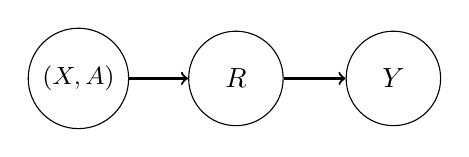
\begin{tikzpicture}

\node[circle,draw, minimum size=1.2cm] (R0) at (0,0) {\begin{small}$(X, A)$\end{small}
};
\node[circle,draw, minimum size=1.2cm] (R1) at (2,0) {$R$};
\node[circle,draw, minimum size=1.2cm] (Y) at (4,0) {$Y$};

\path[->, thick] (R0) edge (R1);
\path[->, thick] (R1) edge (Y);

\end{tikzpicture}
\caption{Bayesian network corresponding to Assumption \ref{assum:indep-general}.}
\label{fig:embedding_single}
%
%
\end{figure}
As illustrated in Figure \ref{fig:embedding_single}, Assumption \ref{assum:indep-general} means that the embedding $R$ fully mediates every possible effect of $(X, A)$ on $Y$. The generalised MIPS estimator $\hat{\theta}_{\textup{G-MIPS}}$ of target policy value, $\Etar[Y]$, is defined as
\[
\hat{\theta}_{\textup{G-MIPS}} \coloneqq \frac{1}{n}\sum_{i=1}^n \frac{\ptar(r_i)}{\pbeh(r_i)}\, y_i,
\]
where $\pbeh(r)$ denote the density of $R$ under the behaviour policy (likewise for $\ptar(r)$). Under assumption \ref{assum:indep-general}, $\hat{\theta}_{\textup{G-MIPS}}$ provides an unbiased estimator of target policy value. 
Similar to Lemma \ref{lemma:weights-est}, the density ratio $\frac{\ptar(r)}{\pbeh(r)}$ can be estimated by solving the regression problem
\begin{align}
    \arg \min_f \Ebeh \left(\frac{\tar(A\mid X)}{\beh(A\mid X)} - f\left(R\right)\right)^2. \label{eq:embedding-ratio-estimation}
\end{align}

\subsection{Variance reduction of G-MIPS estimator}\label{app:gmips-var-reduction}
By only considering the shift in the embedding $R$, the G-MIPS estimator achieves a lower variance relative to the vanilla IPW estimator. The following result, which is a straightforward extension of \cite[Theorem 3.6]{saito2022off}, formalises this.

\begin{proposition}[Variance reduction of G-MIPS]\label{prop:mips_var_reduction}
    When the ratios $\rho(a, x)$ and $\frac{\ptar(r)}{\pbeh(r)}$ are known exactly then under Assumption \ref{assum:indep-general}, we have that $\Ebeh[\thetaipw] = \Ebeh[\hat{\theta}_{\textup{G-MIPS}}] = \Etar[Y]$. Moreover,
\begin{align*}
     \Vbeh[\thetaipw] - \Vbeh[\hat{\theta}_{\textup{G-MIPS}}]
    \geq \frac{1}{n}\Ebeh \left[ \E[Y^2\mid R] \Vbeh[\rho(A, X)\mid R] \right] \geq 0.
\end{align*}
\end{proposition}

\begin{proof}[Proof of Proposition \ref{prop:mips_var_reduction}]
The following proof, which is included for completeness, is a straightforward extension of \cite[Theorem 3.6]{saito2022off}. 
\begin{align*}
    &n (\Vbeh[\thetaipw] - \Vbeh[\hat{\theta}_{\textup{MIPS}}])\\
    &\quad= \Vbeh\left[\frac{\tar(A|X)}{\beh(A|X)}\,Y\right] - \Vbeh\left[\frac{\ptar(R)}{\pbeh(R)}\,Y \right]\\
     &\quad= \Vbeh\left[\Ebeh\left[\frac{\tar(A|X)}{\beh(A|X)}\,Y \Bigg| R\right]\right] + \Ebeh\left[ \Vbeh\left[\frac{\tar(A|X)}{\beh(A|X)}\,Y\Bigg| R \right]\right] - \Vbeh\left[\Ebeh\left[ \frac{\ptar(R)}{\pbeh(R)}\,Y \Bigg| R\right]\right]\\
     &\qquad- \Ebeh\left[\Vbeh\left[ \frac{\ptar(R)}{\pbeh(R)}\,Y \Bigg| R\right]\right]
\end{align*}
Now using the conditional independence Assumption \ref{assum:indep-general}, the first term on the RHS above becomes,
\begin{align*}
    \Vbeh\left[\Ebeh\left[\frac{\tar(A|X)}{\beh(A|X)}\,Y \Bigg| R\right]\right] &= \Vbeh\left[\Ebeh\left[\frac{\tar(A|X)}{\beh(A|X)}\Bigg| R\right]\,\Ebeh\left[Y | R\right]\right]\\
    &= \Vbeh\left[\frac{\ptar(R)}{\pbeh(R)}\,\Ebeh\left[Y | R\right]\right],
\end{align*}
where in the last step above we use the fact that
\begin{align*}
    \Ebeh\left[\frac{\tar(A|X)}{\beh(A|X)}\Bigg| R\right] = \frac{\ptar(R)}{\pbeh(R)}.
\end{align*}
Putting this together, we get that
\begin{align}
    &n (\Vbeh[\thetaipw] - \Vbeh[\hat{\theta}_{\textup{MIPS}}]) \nonumber\\ 
    &\quad= \Ebeh\left[ \Vbeh\left[\frac{\tar(A|X)}{\beh(A|X)}\,Y\Bigg| R \right]\right] - \Ebeh\left[\Vbeh\left[ \frac{\ptar(R)}{\pbeh(R)}\,Y \Bigg| R\right]\right]. \label{eq:variance-difference}
\end{align}
Since we have that 
\begin{align*}
    \Ebeh\left[\frac{\tar(A|X)}{\beh(A|X)}\,Y\Bigg| R \right] = \Ebeh\left[\frac{\tar(A|X)}{\beh(A|X)}\Bigg| R \right]\,\Ebeh\left[Y| R \right] = \frac{\ptar(R)}{\pbeh(R)}\,\Ebeh\left[Y| R \right],
\end{align*}
Eq. \eqref{eq:variance-difference} becomes,
\begin{align*}
    &\Ebeh\left[ \Vbeh\left[\frac{\tar(A|X)}{\beh(A|X)}\,Y\Bigg| R \right]\right] - \Ebeh\left[\Vbeh\left[ \frac{\ptar(R)}{\pbeh(R)}\,Y \Bigg| R\right]\right] \\
    &\quad= \Ebeh\left[ \Ebeh\left[ \left(\frac{\tar(A|X)}{\beh(A|X)}\,Y \right)^2\Bigg| R  \right] - \Ebeh\left[ \left(\frac{\ptar(R)}{\pbeh(R)}\,Y \right)^2\Bigg| R \right] \right]\\
    &\quad= \Ebeh\left[ \Ebeh\left[ \left(\frac{\tar(A|X)}{\beh(A|X)} \right)^2 \Bigg| R  \right] \, \Ebeh\left[Y^2 | R  \right] - \left(\frac{\ptar(R)}{\pbeh(R)}\right)^2\,\Ebeh\left[Y^2 | R \right] \right]\\
    &\quad= \Ebeh\left[\Ebeh\left[Y^2 | R \right]\, \left( \Ebeh\left[ \left(\frac{\tar(A|X)}{\beh(A|X)} \right)^2 \Bigg| R  \right] - \left(\Ebeh\left[ \frac{\tar(A|X)}{\beh(A|X)} \Bigg| R  \right]\right)^2\, \right) \right]\\
    &\quad=\Ebeh\left[\Ebeh\left[Y^2 | R \right]\, \Vbeh\left[\frac{\tar(A|X)}{\beh(A|X)} \Bigg| R \right]\right].
\end{align*}
\end{proof}

\paragraph{Intuition}
Here, $R$ contains all relevant information regarding the outcome $Y$. Moreover, intuitively $R$ can be thought of as the state obtained by `filtering out' relevant information about $Y$ from $(X, A)$. Therefore, $R$ contains less `redundant' information regarding the outcome $Y$ as compared to the covariate-action pair $(X, A)$. As a result, the G-MIPS estimator which only considers the shift in the marginal distribution of $R$ due to the policy shift is more efficient than the IPW estimator, which considers the shift in the joint distribution of $(X, A)$ instead.
In fact, as the amount of `redundant' information regarding $Y$ decreases in the embedding $R$, the G-MIPS estimator becomes increasingly efficient with decreasing variance. We formalise this as follows:
\begin{assumption}\label{assum:two-embeddings}
    Assume there exist embeddings $R^{(1)}, R^{(2)}$ of the covariate-action pair $(X, A)$, with Bayesian network shown in Figure \ref{fig:embedding_double}. 
    This corresponds to the following conditional independence assumptions:
    \[
    R^{(2)} \indep (X, A) \mid R^{(1)}, \qquad \textup{and} \qquad Y \indep (R^{(1)}, X, A) \mid R^{(2)}.
    \]
\end{assumption}
\begin{figure}[h!]
\centering
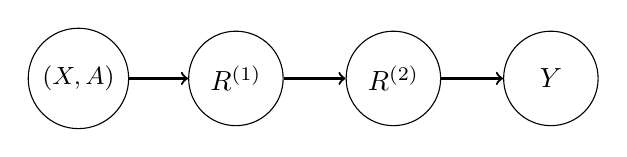
\begin{tikzpicture}

\node[circle,draw, minimum size=1.2cm] (R0) at (0,0) {\begin{small}$(X, A)$\end{small}};
\node[circle,draw, minimum size=1.2cm] (R1) at (2,0) {$R^{(1)}$};
\node[circle,draw, minimum size=1.2cm] (R2) at (4,0) {$R^{(2)}$};
\node[circle,draw, minimum size=1.2cm] (Y) at (6,0) {$Y$};

\path[->, thick] (R0) edge (R1);
\path[->, thick] (R1) edge (R2);
\path[->, thick] (R2) edge (Y);

\end{tikzpicture}
\caption{Bayesian network corresponding to Assumption \ref{assum:two-embeddings}.}
\label{fig:embedding_double}
\end{figure}  
%
We can define G-MIPS estimators for these embeddings to obtain unbiased OPE estimators under Assumption \ref{assum:two-embeddings} as follows:
\[    \hat{\theta}^{(j)}_{\textup{G-MIPS}} \coloneqq \frac{1}{n}\sum_{i=1}^n \frac{\ptar(r_i^{(j)})}{\pbeh(r_i^{(j)})}\, y_i,
\]
for $j\in \{1, 2\}$. Here, $\frac{\ptar(r^{(j)})}{\pbeh(r^{(j)})}$ is the ratio of marginal densities of $R^{(j)}$ under target and behaviour policies. 
We next show that the variance of $\hat{\theta}^{(j)}_{\textup{G-MIPS}}$ decreases with increasing $j$.
\begin{proposition}\label{prop:mips_generalised}
    When the ratios $\rho(a, x)$, $w(y)$ and $\frac{\ptar(r^{(j)})}{\pbeh(r^{(j)})}$ are known exactly for $j \in \{1, 2\}$, then under Assumption \ref{assum:two-embeddings} we get that
    \[
    \Ebeh[\thetaipw] = \Ebeh[\hat{\theta}^{(1)}_{\textup{G-MIPS}}] = \Ebeh[\hat{\theta}^{(2)}_{\textup{G-MIPS}}] = \Ebeh[\thetamr] = \Etar[Y].
    \]
    Moreover, 
    \[
    \Vbeh[\thetaipw] \geq \Vbeh[\hat{\theta}^{(1)}_{\textup{G-MIPS}}] \geq  \Vbeh[\hat{\theta}^{(2)}_{\textup{G-MIPS}}] \geq \Vbeh[\thetamr].
    \]
\end{proposition}
\begin{proof}[Proof of Proposition \ref{prop:mips_generalised}]
    First, we prove that the G-MIPS estimators are unbiased using induction on $j$. We define $R^{(0)} \coloneqq (X, A)$ and $\hat{\theta}^{(0)}_{\textup{G-MIPS}}$ defined as
    \[
    \hat{\theta}^{(0)}_{\textup{G-MIPS}} \coloneqq \frac{1}{n}\sum_{i=1}^n \frac{\ptar(r_i^{(0)})}{\pbeh(r_i^{(0)})}\, y_i,
    \]
    recovers the IPW estimator $\thetaipw$. When $j=0$, we know that $\hat{\theta}^{(0)}_{\textup{G-MIPS}} = \thetaipw$ is unbiased. 
    Now, assume that $\Ebeh[\hat{\theta}^{(j)}_{\textup{G-MIPS}}] = \Etar[Y]$.

    Conditional on $R^{(j)}$, $R^{(j+1)}$ does not depend on the policy. Therefore, 
    \begin{align*}
        \frac{\ptar(r^{(j)})}{\pbeh(r^{(j)})} = \frac{\ptar(r^{(j)})\,p(r^{(j+1)}\mid r^{(j)}) }{\pbeh(r^{(j)})\,p(r^{(j+1)}\mid r^{(j)})} = \frac{\ptar(r^{(j)}, r^{(j+1)})}{\pbeh(r^{(j)}, r^{(j+1)})}.
    \end{align*}
    And therefore,
    \begin{align*}
        \frac{\ptar(r^{(j+1)})}{\pbeh(r^{(j+1)})} &= \int_{r^{(j)}} \frac{\ptar(r^{(j)}, r^{(j+1)})}{\pbeh(r^{(j)}, r^{(j+1)})} \, \pbeh(r^{(j)} \mid r^{(j+1)}) \,\mathrm{d} r^{(j)}\\ 
        &= \int_{r^{(j)}} \frac{\ptar(r^{(j)})}{\pbeh(r^{(j)})} \,\pbeh(r^{(j)} \mid r^{(j+1)}) \,\mathrm{d} r^{(j)}\\ 
        &= \Ebeh\left[\frac{\ptar(R^{(j)})}{\pbeh(R^{(j)})} \Bigg|  R^{(j+1)}=r^{(j+1)}\right].
    \end{align*}
    Using this and the fact that $R^{(j)}\indep Y \mid R^{(j+1)}$, we get that
    \begin{align*}
        \Ebeh\left[\hat{\theta}^{(j+1)}_{\textup{G-MIPS}} \right] &= \Ebeh\left[\frac{\ptar(R^{(j+1)})}{\pbeh(R^{(j+1)})}\, Y \right]\\
        &= \Ebeh\left[\frac{\ptar(R^{(j+1)})}{\pbeh(R^{(j+1)})}\, \Ebeh[Y| R^{(j+1)}] \right]\\
        &= \Ebeh\left[\Ebeh\left[\frac{\ptar(R^{(j)})}{\pbeh(R^{(j)})} \Bigg|  R^{(j+1)}\right]\, \Ebeh[Y| R^{(j+1)}] \right] \\
        &= \Ebeh\left[\Ebeh\left[\frac{\ptar(R^{(j)})}{\pbeh(R^{(j)})} \, Y \Bigg|  R^{(j+1)}\right]\right]\\
        &= \Ebeh\left[ \frac{\ptar(R^{(j)})}{\pbeh(R^{(j)})} \, Y \right]\\
        &= \Ebeh\left[\hat{\theta}^{(j)}_{\textup{G-MIPS}} \right] = \Etar[Y].
    \end{align*}
    Next, to prove the variance result we consider the difference
    \begin{align*}
        &\Vbeh[\hat{\theta}^{(j)}_{\textup{G-MIPS}}] - \Vbeh[\hat{\theta}^{(j+1)}_{\textup{G-MIPS}}] \\
        &= \frac{1}{n}\left(\Vbeh\left[\frac{\ptar(R^{(j)})}{\pbeh(R^{(j)})}\, Y\right] - \Vbeh\left[\frac{\ptar(R^{(j+1)})}{\pbeh(R^{(j+1)})}\, Y\right]\right) \\
        %
        &= \frac{1}{n}\Bigg(\Vbeh\left[ \Ebeh\left[\frac{\ptar(R^{(j)})}{\pbeh(R^{(j)})}\, Y \Bigg| R^{(j+1)} \right] \right] + \Ebeh\left[ \Vbeh\left[\frac{\ptar(R^{(j)})}{\pbeh(R^{(j)})}\, Y \Bigg| R^{(j+1)} \right] \right] \\
        &\qquad- \Vbeh\left[\frac{\ptar(R^{(j+1)})}{\pbeh(R^{(j+1)})}\, \Ebeh[Y\mid R^{(j+1)}]\right] - \Ebeh \left[\left(\frac{\ptar(R^{(j+1)})}{\pbeh(R^{(j+1)})}\right)^2\,\Vbeh[Y\mid R^{(j+1)}] \right] \Bigg)
    \end{align*}
    where in the last step we use the law of total variance. Now, using the fact that $R^{(j)}\indep Y \mid R^{(j+1)}$, we can rewrite the expression above as
    \begin{align*}
        &= \frac{1}{n}\Bigg(\Vbeh\left[ \Ebeh\left[\frac{\ptar(R^{(j)})}{\pbeh(R^{(j)})}\Bigg| R^{(j+1)} \right]\, \Ebeh[Y | R^{(j+1)} ] \right] + \Ebeh\left[ \Vbeh\left[\frac{\ptar(R^{(j)})}{\pbeh(R^{(j)})}\, Y \Bigg| R^{(j+1)} \right] \right] \\
        &\qquad- \Vbeh\left[\frac{\ptar(R^{(j+1)})}{\pbeh(R^{(j+1)})}\, \Ebeh[Y\mid R^{(j+1)}]\right] - \Ebeh \left[\left(\frac{\ptar(R^{(j+1)})}{\pbeh(R^{(j+1)})}\right)^2\,\Vbeh[Y\mid R^{(j+1)}] \right] \Bigg)\\
        &= \frac{1}{n}\Bigg( \Ebeh\left[ \Vbeh\left[\frac{\ptar(R^{(j)})}{\pbeh(R^{(j)})}\, Y \Bigg| R^{(j+1)} \right] \right] - \Ebeh \left[\left(\frac{\ptar(R^{(j+1)})}{\pbeh(R^{(j+1)})}\right)^2\,\Vbeh[Y\mid R^{(j+1)}] \right]\Bigg).
    \end{align*}
    Moreover, again using the conditional independence $R^{(j)}\indep Y \mid R^{(j+1)}$, we can expand the first term in the expression above as follows:
    %
    %
    %
    %
    %
    \begin{align*}
        \Ebeh\left[ \Vbeh\left[\frac{\ptar(R^{(j)})}{\pbeh(R^{(j)})}\, Y \Bigg| R^{(j+1)} \right] \right] &=
        \Ebeh\Bigg[ \Ebeh\left[\frac{\ptar^2(R^{(j)})}{\pbeh^2(R^{(j)})} \Bigg| R^{(j+1)} \right]\,\Ebeh[Y^2 | R^{(j+1)}] \\
        &\qquad- \left(\Ebeh\left[\frac{\ptar(R^{(j)})}{\pbeh(R^{(j)})} \Bigg| R^{(j+1)} \right] \Ebeh[Y | R^{(j+1)}] \right)^2 \Bigg]\\
        &\geq 
        \Ebeh\Bigg[ \left(\Ebeh\left[\frac{\ptar(R^{(j)})}{\pbeh(R^{(j)})} \Bigg| R^{(j+1)} \right]\right)^2 \,\Ebeh[Y^2 | R^{(j+1)}] \\
        &\qquad- \left(\frac{\ptar(R^{(j+1)})}{\pbeh(R^{(j+1)})} \Ebeh[Y | R^{(j+1)}] \right)^2 \Bigg]\\
        &= \Ebeh\Bigg[ \left(\frac{\ptar(R^{(j+1)})}{\pbeh(R^{(j+1)})}\right)^2 \, \Vbeh[Y\mid R^{(j+1)}] \Bigg].
    \end{align*}
    Here, to get the inequality above, we use the fact that $\E[X^2] \geq (\E[X])^2$. Putting this together, we get that $\Vbeh[\hat{\theta}^{(j)}_{\textup{G-MIPS}}] - \Vbeh[\hat{\theta}^{(j+1)}_{\textup{G-MIPS}}] \geq 0$.

    Moreover, the result $\Vbeh[\hat{\theta}^{(2)}_{\textup{G-MIPS}}] \geq \Vbeh[\thetamr]$ follows straightforwardly from above by defining $R^{(3)} \coloneqq Y$. Then, the embeddings satisfy the causal structure 
    \[
    R^{(0)} \rightarrow R^{(1)} \rightarrow R^{(2)}  \rightarrow R^{(3)} \rightarrow Y.
    \]
    Using the result above, we know that $\Vbeh[\hat{\theta}^{(2)}_{\textup{G-MIPS}}] \geq \Vbeh[\hat{\theta}^{(3)}_{\textup{G-MIPS}}]$. But now it is straightforward to see that $\hat{\theta}^{(3)}_{\textup{G-MIPS}} = \thetamr$, and the result follows.
\end{proof}

\paragraph{Intuition}
Here, $R^{(j+1)}$ can be thought of as the embedding obtained by `filtering out' relevant information about $Y$ from $R^{(j)}$. As such, the amount of `redundant' information regarding the outcome $Y$ decreases successively along the sequence $R^{(0)} (\coloneqq (X, A)), R^{(1)}, R^{(2)}$. As a result, the G-MIPS estimators which only consider the shift in the marginal distributions of $R^{(j)}$ due to policy shift become increasingly efficient with decreasing variance as $j$ increases. Define the representation $R^{(3)} \coloneqq Y$, then the corresponding G-MIPS estimator reduces to the MR estimator, i.e., $\hat{\theta}^{(3)}_{\textup{G-MIPS}} = \thetamr$. Moreover, this estimator has minimum variance among all the G-MIPS estimators $\{\hat{\theta}^{(j)}_{\textup{G-MIPS}}\}_{0\leq j\leq k}$, as the representation $R^{(3)}$ contains precisely the least amount of information necessary to obtain the outcome $Y$. In other words, $Y$ itself serves as the `best embedding' of covariate-action pair $R^{(0)}$ which contains all relevant information regarding $Y$. We verify this empirically in Appendix \ref{subsec:mips-empirical} by reproducing the experimental setup in \cite{saito2022off} along with the MR baseline. Additionally, the MR estimator does not rely on assumptions like \ref{assum:indep-general} for unbiasedness. 

In addition to this, solving the regression problem in Eq. \eqref{eq:embedding-ratio-estimation} will typically be more difficult when $R$ is higher dimensional (as is likely to be the case for many choices of embeddings $R$), leading to high bias. In contrast, for MR the embedding $R=Y$ is one dimensional and therefore the regression problem is significantly easier to solve and yields lower bias. Our empirical results in Appendix \ref{app:experiments} confirm this.

\subsection{Doubly robust G-MIPS estimators}
Consider the setup for the G-MIPS estimator shown in Figure \ref{fig:embedding_single}. In this case, we can derive a doubly robust extension of the G-MIPS estimator, denoted as GM-DR, which uses an estimate of the conditional mean $\tilde{\mu}(r) \approx \E[Y\mid R=r]$ as a control variate to decrease the variance of G-MIPS estimator. This can be explicitly written as follows:
\begin{align}
\thetagmdr \coloneqq \frac{1}{n} \sum_{i=1}^n \frac{\ptar(r_i)}{\pbeh(r_i)}\,(y_i - \tilde{\mu}(r_i)) + \tilde{\eta}(\tar). \label{eq:gmips-dr}    
\end{align}
where $\tilde{\eta}(\tar) = \frac{1}{n} \sum_{i=1}^n \sum_{r' \in \mathcal{R}} \tilde{\mu}(r') \, \ptar(r' \mid x_i)$ is the analogue of the direct method. Here, $\mathcal{R}$ denotes the space of the possible of the representations $R$\footnote{the $\sum_{r' \in \mathcal{R}}$ can be replaced with $\int_{r' \in \mathcal{R}} \mathrm{d}r'$ when $\mathcal{R}$ is continuous}. Moreover, given the density $p(r \mid x, a)$, we can compute $\ptar(r\mid x)$ using
\[
\ptar(r\mid x) = \sum_{a' \in \Aspace} p(r \mid x, a')\,\tar(a'\mid x).
\]
It is straightforward to extend ideas from \cite{dudik2014doubly} to show that estimator $\thetagmdr$ is doubly robust in that it will yield accurate value estimates if either the importance weights $\frac{\ptar(r)}{\pbeh(r)}$ or the outcome model $\tilde{\mu}(r)$ is well estimated. 

\paragraph{There is no analogous DR extension of the MR estimator}
A consequence of considering the embedding $R=Y$ (as in MR) is that in this case we do not have an analogous doubly robust extension as above. To see why this is the case, note that when $R=Y$, we get that $\tilde{\mu}(r) = \E[Y\mid R=r] = \E[Y\mid Y=y] = y$. If we substitute this $\tilde{\mu}(r)$ in \eqref{eq:gmips-dr}, we are simply left with $\tilde{\eta}(\tar)$ on the right hand side (as the first term cancels out). This means that the resulting estimator does not retain the doubly robust nature as we no longer obtain an accurate estimate if either the outcome model or the importance ratios are well estimated.
%
%


%
\section{Application to causal inference}\label{app:causal-inference}
In this section, we investigate the application of the MR estimator for the estimation of average treatment effect (ATE). In this setting, we suppose that $\Aspace = \{0, 1\}$, and the goal is to estimate ATE defined as follows:
\[
\ate \coloneqq \E[Y(1)-Y(0)]
\]
Here, we use the potential outcomes notation \citep{robins1986new} to denote the outcome under a deterministic policy $\tar(a'\mid x) = \mathbbm{1}(a'=a)$ as $Y(a)$. 

Specifically, the IPW estimator applied to ATE estimation yields:
\[
\ateipw = \frac{1}{n} \sum_{i=1}^n \rho_{\ate}(a_i, x_i) \times y_i,
\]
where 
\[
\rho_{\ate}(a, x) \coloneqq \frac{\mathbbm{1}(a=1) - \mathbbm{1}(a=0)}{\beh (a|x)}.
\]
Similarly, the MR estimator can be written as
\[
\atemr = \frac{1}{n}\sum_{i=1}^n w_{\ate}(y_i)\times y_i, 
\]
where
\[
w_{\ate}(y) = \frac{p_{\pi^{(1)}}(y) - p_{\pi^{(0)}}(y)}{\pbeh(y)},
\] 
and $\pi^{(a)}(a'\mid x) \coloneqq \mathbbm{1}(a'=a)$ for $a\in \{0,1\}$.

Again, using the fact that $w_{\ate}(Y) \eqas \E[\rho_{\ate}(A, X)\mid Y]$, we can obtain $w_{\ate}$ by minimising a simple mean-squared loss:
\begin{align*}
    w_{\ate} =\arg \min_{f} \Ebeh \Big[\frac{\mathbbm{1}(A=1)- \mathbbm{1}(A=0)}{\beh (A|X)}-f(Y)\Big]^2.
\end{align*}
\begin{proposition}[Variance comparison with IPW ATE estimator]\label{prop:ate_variance}
When the weights $\rho_{\ate}(a, x)$ and $w_{\ate}(y)$ are known exactly, we have that $\V[\atemr] \leq \V[\ateipw]$. Specifically,
\begin{align*}
    \V[\ateipw] - \V[\atemr] = \frac{1}{n}\E\left[ \V\left[\rho_{\ate}(A, X) | Y \right]\,Y^2 \right] \geq 0.
\end{align*}
\end{proposition}
\begin{proof}[Proof of Proposition \ref{prop:ate_variance}] We have
\begin{align}
    \V[\ateipw] - \V[\atemr] &= \frac{1}{n}\left( \V[\rho_{\ate}(A, X)\, Y] - \V[w_{\ate}(Y)\,Y] \right). \label{eq:variance_ate_ipw_minus_mr}
\end{align}
Using the tower law of variance, we get that
\begin{align*}
    \V[\rho_{\ate}(A, X)\, Y] 
    &= \V[\E[\rho_{\ate}(A, X)\,  Y\mid Y]] + \E[\V[\rho_{\ate}(A, X)\, Y\mid Y]]\\
    &= \V[\E[\rho_{\ate}(A, X)\mid Y]\,  Y] + \E[\V[\rho_{\ate}(A, X)\mid Y]\,Y^2]\\
    &= \V[w_{\ate}(Y)\,Y] + \E[\V[\rho_{\ate}(A, X)\mid Y]\,Y^2].
\end{align*}
Putting this together with \eqref{eq:variance_ate_ipw_minus_mr} we obtain,
\begin{align*}
    \V[\ateipw] - \V[\atemr] &= \frac{1}{n} \E[\V[\rho_{\ate}(A, X)\mid Y]\,Y^2],
\end{align*}
which straightforwardly leads to the result.
\end{proof}

Given the above definitions, the IPW estimator for $\E[Y(a)]$ would only consider datapoints with $A=a$, as it weights the samples using the policy ratios $\mathbbm{1}(A=a)/\beh(A|X)$ which are only non-zero when $A=a$. 
This is however not the case with the MR estimator, as it uses the weights $\ptar(Y)/\pbeh(Y)$ which are not necessarily zero for $A\neq a$. Therefore, MR uses all evaluation datapoints $\D$ when estimating $\E[Y(a)]$. The MR estimator therefore leads to a more efficient use of evaluation data in this example. 
%
%

Likewise, the doubly robust (DR) estimator applied to ATE estimation yields,
\begin{align*}
    \atedr \coloneqq \frac{1}{n} \sum_{i=1}^n \rho_{\ate}(a_i, x_i)\,\left(y_i - \hat{\mu}(a_i, x_i)\right) + \frac{1}{n} \sum_{i=1}^n \left( \hat{\mu}(1, x_i)-  \hat{\mu}(0, x_i)\right),
\end{align*}
where $\hat{\mu}(a, x)\approx \E[Y\mid X=x, A=a]$. 
Like in classical off-policy evaluation, DR yields an accurate estimator of ATE when either the weights $\rho_{\ate}(a, x)$ or the outcome model i.e., $\hat{\mu}(a, x) = \E[Y\mid X=x, A=a]$, are well estimated.
However, despite this doubly robust nature of the estimator, we can show that the variance of the DR estimator may be higher than that of the MR estimator in many cases. The following result formalises this variance comparison between the DR and MR estimators, and is analogous to the result in Proposition \ref{prop:var_dr} derived for classical off-policy evaluation. 
\begin{proposition}[Variance comparison with DR ATE estimator]\label{prop:ate_var_dr}
    When the weights $\rho_{\ate}(a, x)$ and $w_{\ate}(y)$ are known exactly,
    \begin{align*}
    &\V[\atedr] - \V[\atemr]\\
    &\qquad \qquad \qquad \geq \frac{1}{n}\E \left[ \V\left[ \rho_\ate(A, X)\,Y \mid Y \right] -  \V\left[ \rho_\ate(A, X)\mu(A, X) \mid X \right] \right],
\end{align*}
where $\mu(A, X) \coloneqq \E[Y\mid X, A]$.
\end{proposition}

\begin{proof}[Proof of Proposition \ref{prop:ate_var_dr}]
Using the law of total variance, we get that
\begin{align*}
    n\,\V[\atedr] &= \V[\rho_\ate(A, X)\,(Y -\hat{\mu}(A, X)) + (\hat{\mu}(1, X) - \hat{\mu}(0, X))]\\
    &= \V[ \E[\rho_\ate(A, X)\,(Y -\hat{\mu}(A, X)) + (\hat{\mu}(1, X) - \hat{\mu}(0, X))\mid X, A]] \\
    &\qquad+ \E[\V[\rho_\ate(A, X)\,(Y -\hat{\mu}(A, X)) + (\hat{\mu}(1, X) - \hat{\mu}(0, X))\mid X, A]]\\
    &= \V[ \rho_\ate(A, X)\,(\mu(A, X) -\hat{\mu}(A, X)) + (\hat{\mu}(1, X) - \hat{\mu}(0, X))]\\
    &\qquad+ \E[\rho^2_\ate(A, X)\V[Y\mid X, A]].
\end{align*}
    Again, using the law of total variance we can rewrite the first term on the RHS above as,
    \begin{align*}
        &\V[ \rho_\ate(A, X)\,(\mu(A, X) -\hat{\mu}(A, X)) + (\hat{\mu}(1, X) - \hat{\mu}(0, X))]\\
        &\quad= \V[\E[ \rho_\ate(A, X)\,(\mu(A, X) -\hat{\mu}(A, X)) + (\hat{\mu}(1, X) - \hat{\mu}(0, X))\mid  X]] \\
        &\qquad+ \E[\V[ \rho_\ate(A, X)\,(\mu(A, X) -\hat{\mu}(A, X)) + (\hat{\mu}(1, X) - \hat{\mu}(0, X))\mid  X]] \\
        &\quad\geq  \V[\E[ \rho_\ate(A, X)\,(\mu(A, X) -\hat{\mu}(A, X)) + (\hat{\mu}(1, X) - \hat{\mu}(0, X))\mid  X]]\\
        &\quad=  \V[\E[ \rho_\ate(A, X)\,(\mu(A, X) -\hat{\mu}(A, X)) + \rho_\ate(A, X)\,\hat{\mu}(A, X)\mid  X]]\\
        &\quad=  \V[\E[ \rho_\ate(A, X)\,\mu(A, X)\mid  X]],
    \end{align*}
    where, in the second last step above we use the fact that 
    \[
    \E[\rho_\ate(A, X)\,\hat{\mu}(A, X)\mid  X] = \hat{\mu}(1, X) - \hat{\mu}(0, X).
    \]

    Putting this together, we get that
    \begin{align*}
        n\,\V[\atedr] \geq \V[\E[ \rho_\ate(A, X)\,\mu(A, X)\mid  X]] + \E[\rho^2_\ate(A, X)\V[Y\mid X, A]].
    \end{align*}
    Therefore, 
    \begin{align*}
        &n\,(\V[\atedr] - \V[\atemr]) \\
        &\quad\geq \V[\E[ \rho_\ate(A, X)\,\mu(A, X)\mid  X]] + \E[\rho^2_\ate(A, X)\V[Y\mid X, A]] - \V[w_\ate(Y)\,Y]\\
        &\quad= \V[\E[ \rho_\ate(A, X)\,\mu(A, X)\mid  X]] + \E[\V[\rho_\ate(A, X)\,Y\mid X, A]] - \V[w_\ate(Y)\,Y]\\
        &\quad= \V[\E[ \rho_\ate(A, X)\,\mu(A, X)\mid  X]] + \V[\rho_\ate(A, X)\, Y] - \V[\E[\rho_\ate(A, X)\,Y\mid X, A]]\\
        &\qquad- \V[w_\ate(Y)\,Y]\\
        &\quad= \V[\E[ \rho_\ate(A, X)\,\mu(A, X)\mid  X]] + \V[\E[\rho_\ate(A, X)\mid Y]\, Y] + \E[\V[\rho_\ate(A, X)\mid Y]\,Y^2]\\
        &\qquad- \V[\E[\rho_\ate(A, X)\,Y\mid X, A]]- \V[w_\ate(Y)\,Y]\\
        &\quad= \V[\E[ \rho_\ate(A, X)\,\mu(A, X)\mid  X]] + \V[w_\ate(Y)\, Y] + \E[\V[\rho_\ate(A, X)\mid Y]\,Y^2]\\
        &\qquad- \V[\E[\rho_\ate(A, X)\,Y\mid X, A]]- \V[w_\ate(Y)\,Y]\\
        &\quad= \V[\E[ \rho_\ate(A, X)\,\mu(A, X)\mid  X]]- \V[\E[\rho_\ate(A, X)\,Y\mid X, A]] + \E[\V[\rho_\ate(A, X)\mid Y]\,Y^2]\\
        &\quad= \V[\rho_\ate(A, X)\,\mu(A, X)] - \E[\V[\rho_\ate(A, X)\,\mu(A, X)\mid  X]] - \V[\rho_\ate(A, X)\,\mu(A, X)]\\
        &\qquad+ \E[\V[\rho_\ate(A, X)\mid Y]\,Y^2]\\
        &\quad= \E \left[ \V\left[ \rho_\ate(A, X) \mid Y \right]\, Y^2 -  \V\left[ \rho_\ate(A, X)\mu(A, X) \mid X \right] \right].
        %
    \end{align*}
\end{proof}

Proposition \ref{prop:ate_var_dr} shows that if $\V\left[Y\, \rho_\ate(A, X) \mid Y \right]$ is greater than the conditional variance $\V\left[ \rho_\ate(A, X)\mu(A, X) \mid X \right]$ on average, the variance of the MR estimator will be less than that of the DR estimator. Intuitively, this is likely to happen when the dimension of context space $\Xspace$ is high because in this case, the conditional variance over $X$ and $A$, $\V\left[Y\, \rho_\ate(A, X) \mid Y \right]$ is likely to be greater than the conditional variance over $A$, $\V\left[ \rho_\ate(A, X)\mu(A, X) \mid X \right]$.

%
\section{Experimental Results}\label{app:experiments}
In this section, we provide additional experimental details for the results presented in the main text. We also include extensive experimental results to provide further empirical evidence in favour of the MR estimator. 

\paragraph{Computational details}
We ran our experiments on Intel(R) Xeon(R) CPU E5-2690 v4 @ 2.60GHz with 8GB RAM
per core. We were able to use 150 CPUs in parallel to iterate over different configurations and seeds.
However, we would like to note that for each run our algorithms only requires 1 CPU and at most 30 minutes to run as our neural networks are relatively small. Throughout our experiments, whenever the outcome $Y$ was continuous, we used a fully connected neural network with three hidden layers with 512, 256 and 32 nodes respectively (and ReLU activation function) to estimate the weights $\hat{w}(y)$. On the other hand, when the outcome is discrete we can directly estimate $\hat{w}(y) \approx \E[\hat{\rho}(A, X)\mid Y=y]$ by calculating the sample mean of $\hat{\rho}(A, X)$ on samples with $Y=y$. Additionally, for each configuration of parameters in our experiments, we ran experiments for 10 different seeds (in \{0, 1, \ldots, 9\}).

\subsection{Alternative methodology of estimating MR}
In addition to the OPE baselines like IPW, DM and DR estimators considered in the main text, we also include empirically investigate an alternative methodology of estimating MR.
%
Below we describe this methodology, denoted as `MR (alt)', in greater detail:
\subsubsection{MR (alt)}\label{sec:alt-estimation-method}
Recall our definition of MR estimator:
\[
\thetamr \coloneqq \frac{1}{n} \sum_{i=1}^n w(y_i)\,y_i.
\]
In the main text, we propose estimating the weights $w(y)$ first and using this to estimate $\thetamr$ using the above expression. Alternatively, we can estimate $h(y) \coloneqq y\,w(y)$ using 
\begin{align*}
    h = \arg\min_{f} \, \Ebeh \left[ \Bigg(Y\,\frac{\tar(A|X)}{\beh (A|X)}-f(Y)\Bigg)^2\right].
\end{align*}
Subsequently, the MR estimator can be written as:
\[
\thetamr = \frac{1}{n}\sum_{i=1}^n h(y_i).
\]
We refer to this alternative methodology as `MR-alt' and compare it empirically against the original methodology (which we simply refer to as `MR'). 
In general, it is difficult to say which of the two methods will perform better. Intuitively speaking, in cases where the behaviour of the quantity $Y\,\frac{\tar(A|X)}{\beh (A|X)}$ with varying $Y$ is `smoother' than that of $\frac{\tar(A|X)}{\beh (A|X)}$, the alternative method is expected to perform better. Our empirical results in the next sections show that the relative performance of the two methods varies for different data generating mechanisms.

%
%
%
%
%
%
%
%
%

%
%
%
%
%
%
%
%
%
%

\subsection{Synthetic data experiments}\label{subsec:mips-empirical}
Here, we include additional experimental details for the synthetic data experiments presented in Section \ref{sec:exp-synth} for completeness. For this experiment, we use the same setup as the synthetic data experiment in \cite{saito2022off}, reproduced by reusing their code with minor modifications. 


%

\paragraph{Setup}
Here, we sample the $d$-dimensional context vectors $x$ from a standard normal distribution. 
The setup used also includes $3$-dimensional categorical action embeddings $E \in \mathcal{E}$, which are sampled from the following conditional distribution given action $A=a$,
\[
p(e\mid a) = \prod_{k=1}^{3}\frac{\exp{(\alpha_{a, e_{k}})}}{\sum_{e'\in \mathcal{E}_k} \exp{(\alpha_{a, e'})}},
\]
which is independent of the context $X$. $\{\alpha_{a, e_k}\}$ is a set of parameters sampled independently from the standard normal distribution. Each dimension of $\mathcal{E}$ has a cardinality of $10$, i.e., $\mathcal{E}_k = \{1, 2, \dots, 10\}$.

\paragraph{Reward function}
The expected reward is then defined as:
\[
q(x, e) = \sum_{k=1}^{3} \eta_k \cdot (x^T\, M\, x_{e_k} + \theta_x^T\, x + \theta_e^T\, x_{e_k}),
\]
where $M$, $\theta_x$ and $\theta_e$ are parameter matrices or vectors sampled from a uniform distribution with range $[-1, 1]$. $x_{e_k}$ is a context vector corresponding to the $k$-th dimension of the action embedding, which is unobserved to the estimators. $\eta_k$ specifies the importance of the $k$-th dimension of the action embedding, sampled from Dirichlet distribution so that $\sum_{k=1}^{3} \eta_k = 1$. 

\paragraph{Behaviour and target policies}
The behaviour policy $\beh$ is defined by applying the softmax function to $q(x, a) = \E[q(X, E)\mid A=a, X=x]$ as 
\[
\beh(a\mid x) = \frac{\exp{(-q(x, a))}}{\sum_{a'\in \Aspace}\exp{(-q(x, a'))}}.
\]
%

For the target policy, we define the class of parametric policies,
\[
\pi^{\alpha^\ast}(a | x) = \alpha^\ast\,\ind(a = \arg\max_{a'\in \Aspace} q(x, a')) + \frac{1-\alpha^\ast}{|\Aspace|},
\]
where $\alpha^\ast \in [0, 1]$ controls the shift between the behaviour and target policies. As shown in the main text, as $\alpha^\ast \rightarrow 1$, the shift between behaviour and target policies increases.

\paragraph{Baselines}
In the main text, we compare MR with DM, IPW, DR and MIPS estimators. In addition to these baselines, here we also consider Switch-DR \citep{wang2017optimal} and DR with Optimistic Shrinkage (DRos) \citep{su2020doubly}.
Following \cite{saito2022off}, we use the random forest \citep{breiman2001machine} along with 2-fold cross-fitting \citep{newey2018cross} to obtain $\hat{q}(x, e)$ for DR and DM methods.
To estimate $\pbeh(a\mid x, e)$ for MIPS estimator, we use logistic regression. 
We also include the results for MR estimated using the alternative methodology described in Section \ref{sec:alt-estimation-method}. We refer to this as `MR (alt)'.
%

\paragraph{Estimation of behaviour policy $\hatbeh$ and marginal ratio $\hat{w}(y)$}
We do not assume that the true behaviour policy $\beh$ is known, and therefore estimate $\hatbeh$ using the available training data.
For the MR estimator, we estimate the behaviour policy using a random forest classifier trained on 50\% of the training data and use the rest of the training data to estimate the marginal ratios $\hat{w}(y)$ using multi-layer perceptrons (MLP). Moreover, for a fair comparison we use a different behaviour policy estimate $\hatbeh$ for all other baselines which is trained on the entire training data. 


\begin{figure}[h!]
    \centering
	\begin{subfigure}{0.8\textwidth}
	    \centering
	    \includegraphics[width=1\textwidth]{figures/mr/mips_experiments/ope_vs_neval_nac_250_alphatar_0_8_dimc_5000.png}
	    \subcaption{$d=1000$, $n_{a}=100$, $\alpha^\ast = 0.8$}
	    \label{subfig:d-1000-na-250-neval-mips}
	\end{subfigure}\\
	\begin{subfigure}{0.8\textwidth} 
	    \centering
	    \includegraphics[width=1\textwidth]{figures/mr/mips_experiments/ope_vs_neval_nac_100_alphatar_0_8_dimc_1000.png}
	    \subcaption{$d=5000$, $n_{a}=250$, $\alpha^\ast = 0.8$}
	    \label{subfig:d-5000-na-250-neval-08-mips}
	\end{subfigure}\\
	\begin{subfigure}{0.8\textwidth} 
	    \centering
	    \includegraphics[width=1\textwidth]{figures/mr/mips_experiments/ope_vs_neval_nac_250_alphatar_1_0_dimc_5000.png}
	    \subcaption{$d=5000$, $n_{a}=250$, $\alpha^\ast = 1.0$}
	    \label{subfig:d-5000-na-250-neval-1-mips}
	\end{subfigure}
    \caption{MSE with varying size of evaluation dataset $n$ for different choices of parameters.}
    \label{fig:mse-vs-neval-mips}
\end{figure}

\begin{figure}[h!]
    \centering
	\begin{subfigure}{0.8\textwidth}
	    \centering
	    \includegraphics[width=1\textwidth]{figures/mr/mips_experiments/ope_vs_alphatar_dimc_100_neval_100_nac_100_ntrain_100000.png}
	    \subcaption{$d=100$, $n_{a}=100$, $n = 100$}
	    \label{subfig:d-100-na-100-neval-100-alphatar-mips}
	\end{subfigure}\\
	\begin{subfigure}{0.8\textwidth} 
	    \centering
	    \includegraphics[width=1\textwidth]{figures/mr/mips_experiments/ope_vs_alphatar_dimc_100_neval_100_nac_250_ntrain_100000.png}
	    \subcaption{$d=100$, $n_{a}=250$, $n = 100$}
	    \label{subfig:d-100-na-250-neval-100-alphatar-mips}
	\end{subfigure}\\
	\begin{subfigure}{0.8\textwidth} 
	    \centering
	    \includegraphics[width=1\textwidth]{figures/mr/mips_experiments/ope_vs_alphatar_dimc_1000_neval_100_nac_250_ntrain_100000.png}
	    \subcaption{$d=1000$, $n_{a}=250$, $n = 100$}
	    \label{subfig:d-1000-na-250-neval-100-alphatar-mips}
	\end{subfigure}
    \caption{MSE with varying $\alpha^\ast$ for different choices of parameters.}
    \label{fig:mse-vs-alphatar-mips}
\end{figure}

\subsubsection{Results}
For this experiment, the results are computed over 10 different sets of logged data replicated with different seeds, and in Figures \ref{fig:mse-vs-neval-mips} - \ref{fig:mse-vs-nac-mips} we use a total of $m=5000$ training data. 

\paragraph{Varying size of evaluation data $n$}
Figure \ref{fig:mse-vs-neval-mips} shows that MR outperforms the other baselines, in terms of MSE and squared bias, when the number of evaluation data $n\leq 1000$. Additionally, we observe that in this experiment, MR estimated using our original methods (`MR'), yields better results than the alternative method of estimating MR (`MR (alt)'). Moreover, while the variance of DM is lower than that of MR, the DM method has a high bias and consequently a high MSE. We note that while the difference between MSE and variance of MIPS and MR estimators decreases with increasing evaluation data size, MR still outperforms MIPS in terms of both MSE and variance.

\paragraph{Varying $\alpha^\ast$}
Figure \ref{fig:mse-vs-alphatar-mips} shows the results with increasing policy shift. It can be seen that overall MR methods achieve the smallest MSE with increasing policy shift. Moreover, the difference between MSE and variance of MR and IPW/DR methods increases with increasing policy shift, showing that MR performs especially better than these baselines when the difference between behaviour and target policies is large. Similarly, we observe in Figure \ref{fig:mse-vs-alphatar-mips} that as the shift between the behaviour and target policy increases with increasing $\alpha^\ast$, so does the difference between the MSE and variance of MR and the MIPS estimators. This shows that generally MR outperforms MIPS estimator in terms of variance and MSE, and that MR performs especially better than MIPS as the difference between behaviour and target policies increases.

\paragraph{Varying $d$ and $n_a$}
Figures \ref{fig:mse-vs-d-mips} and \ref{fig:mse-vs-nac-mips} show that MR outperforms the other baselines as the context dimensions and/or number of actions increase. In fact, these figures show that MR is significantly robust to increasing dimensions of action and context spaces, whereas baselines like IPW and DR perform poorly in large action spaces.

\paragraph{Varying $m$}
Figure \ref{fig:mse-vs-ntr-mips} shows the results with increasing number of training data $m$. We again observe that the MR methods `MR' and `MR (alt)' outperforms the other baselines in terms of the MSE and squared bias even when the number of training data is low. Moreover, the variance of both the MR estimators continues to improve with increasing number of training data.

In this experiment, we observe that overall `MR (alt)' performs worse than the original MR estimator (`MR' in the figures). However, as we observe in Appendix \ref{sec:app-additional-results}, this does not happen consistently across all experiments, which suggests that the comparative performance of the two MR methods depends on the data generating mechanism. 




\begin{figure}[h!]
    \centering
	\begin{subfigure}{0.8\textwidth}
	    \centering
	    \includegraphics[width=1\textwidth]{figures/mr/mips_experiments/ope_vs_d_nac_20_alphatar_0_8_n_200.png}
	    \subcaption{$n_{a}=20$, $n = 200$, $\alpha^\ast = 0.8$}
	    \label{subfig:na-20-neval-200-alphatar-0-8-d-mips}
	\end{subfigure}\\
	\begin{subfigure}{0.8\textwidth} 
	    \centering
	    \includegraphics[width=1\textwidth]{figures/mr/mips_experiments/ope_vs_d_nac_100_alphatar_0_8_n_200.png}
	    \subcaption{$n_{a}=100$, $n = 200$, $\alpha^\ast = 0.8$}
	    \label{subfig:na-100-neval-200-alphatar-0-8-d-mips}
	\end{subfigure}\\
	\begin{subfigure}{0.8\textwidth} 
	    \centering
	    \includegraphics[width=1\textwidth]{figures/mr/mips_experiments/ope_vs_d_nac_250_alphatar_0_8_n_200.png}
	    \subcaption{$n_{a}=250$, $n = 200$, $\alpha^\ast = 0.8$}
	    \label{subfig:na-250-neval-200-alphatar-0-8-d-mips}
	\end{subfigure}
    \caption{MSE with varying context dimensions $d$ for different choices of parameters.}
    \label{fig:mse-vs-d-mips}
\end{figure}

\begin{figure}[h!]
    \centering
	\begin{subfigure}{0.8\textwidth}
	    \centering
	    \includegraphics[width=1\textwidth]{figures/mr/mips_experiments/ope_vs_nac_dimc_1000_alphatar_0_4_neval_100_ntrain_100000.png}
	    \subcaption{$d=1000$, $n = 100$, $\alpha^\ast = 0.4$}
	    \label{subfig:d-1000-neval-100-alphatar-0-4-nac-mips}
	\end{subfigure}\\
	\begin{subfigure}{0.8\textwidth} 
	    \centering
	    \includegraphics[width=1\textwidth]{figures/mr/mips_experiments/ope_vs_nac_dimc_1000_alphatar_0_8_neval_100_ntrain_100000.png}
	    \subcaption{$d=1000$, $n = 100$, $\alpha^\ast = 0.8$}
	    \label{subfig:d-1000-neval-100-alphatar-0-8-nac-mips}
	\end{subfigure}\\
	\begin{subfigure}{0.8\textwidth} 
	    \centering
	    \includegraphics[width=1\textwidth]{figures/mr/mips_experiments/ope_vs_nac_dimc_1000_alphatar_1_0_neval_100_ntrain_100000.png}
	    \subcaption{$d=1000$, $n = 100$, $\alpha^\ast = 1.0$}
	    \label{subfig:d-1000-neval-100-alphatar-1-0-nac-mips}
	\end{subfigure}
    \caption{MSE with varying number of actions $n_a$ for different choices of parameters.}
    \label{fig:mse-vs-nac-mips}
\end{figure}

\begin{sidewaystable}[ht]
    \centering
        \caption{Mean-squared error results with 2 standard errors for synthetic data setup considered in Section \ref{sec:exp-synth} with $d=5000$, $n_a = 50$, $\alpha^\ast = 0.8$. We use a fixed budget of datapoints (denoted by $N$) for each baseline and in the case of MR we use $m=2000$ of the available datapoints to estimate $\hat{w}(y)$ and the rest of data to evaluate the MR estimator (i.e. $n = N-2000$ for MR). In contrast, for IPW and MIPS since the importance ratios are already known, we use all of the $N$ datapoints for evaluation of the off-policy value (i.e. $n=N$ for IPW and MIPS).}
    \label{tab:known_ratios}
    \begin{tiny}
    \begin{tabular}{l|llllll}
\toprule
& $N$ & 2800 & 3200 & 6400 & 10000 & 12000 \\
\midrule
\multirow{2}{*}{
\begin{tiny}
\textbf{GT weights $\rho(a, x)$ and estimated reward model $\hat{\mu}(a, x)$}
\end{tiny}}
& DM & 0.137$\pm$0.028 & 0.099$\pm$0.012 & 0.103$\pm$0.012 & 0.093$\pm$0.010 & 0.089$\pm$0.010 \\
\multirow{2}{*}{
\begin{tiny}
($m=2000$ used for training $\hat{\mu}(a, x)$ and $n=N-2000$ 
\end{tiny}}
& DR & 0.227$\pm$0.065 & 0.068$\pm$0.035 & 0.068$\pm$0.022 & \textbf{0.024$\pm$0.011} & 0.045$\pm$0.015 \\
\multirow{2}{*}{
\begin{tiny}
used for evaluation)
\end{tiny}} & DRos & 0.128$\pm$0.027 & 0.072$\pm$0.011 & 0.049$\pm$0.014 & 0.063$\pm$0.014 & 0.051$\pm$0.016 \\
& SwitchDR & 0.128$\pm$0.027 & 0.059$\pm$0.014 & 0.052$\pm$0.013 & 0.061$\pm$0.015 & 0.056$\pm$0.016 \\
\hline
\\
\multirow{2}{*}{
\begin{tiny}
\textbf{GT weights} (all of $N$ datapoints are used for evaluation)
\end{tiny}}
& IPW & 0.237$\pm$0.062 & 0.066$\pm$0.036 & 0.067$\pm$0.021 & 0.025$\pm$0.011 & \textbf{0.044$\pm$0.014} \\
& MIPS & 0.236$\pm$0.062 & 0.065$\pm$0.035 & 0.067$\pm$0.021 & 0.025$\pm$0.011 & \textbf{0.044$\pm$0.014} \\
\hline
\multirow{3}{*}{
\begin{tiny}
\textbf{Estimated weights $\hat{w}(y)$}
\end{tiny}}
\multirow{3}{*}{
\begin{tiny}
($m=2000$ used for training
\end{tiny}} \\
\multirow{3}{*}{
\begin{tiny}
and $n=N-2000$ used for evaluation)
\end{tiny}} 
& MR (Ours) & \textbf{0.045$\pm$0.015} & \textbf{0.042$\pm$0.014} & \textbf{0.048$\pm$0.020} & 0.049$\pm$0.020 & 0.047$\pm$0.016
\\
\\
\bottomrule
\end{tabular}
    \end{tiny}
\end{sidewaystable}
\subsubsection{Known policy ratios $\rho(a, x)$}
Our previous setting of unknown importance policy ratios $\rho(a, x)$ captures a wide variety of real-world applications, ranging from health care to autonomous driving. In addition, to demonstrate the utility of MR in settings with known $\rho(a, x), p(e\mid a, x)$ and unknown $w(y)$ (for our proposed method, MR), we have conducted additional experiments. Here, we use a fixed budget of datapoints (denoted by $N$) for each baseline and for MR we allocate $m=2000$ of the available datapoints to estimate $\hat{w}(y)$ and use the remaining for evaluating the MR estimator (i.e., $n=N-2000$ for MR). In contrast, for IPW and MIPS (since the importance ratios are already known), we use all of the $N$ datapoints to evaluate the off-policy value (i.e. $n=N$ for IPW and MIPS).

The results included in Table \ref{tab:known_ratios} show that MR achieves the smallest MSE among the baselines for $N\leq 6400$. However, we observe that the MSE of IPW, DR and MIPS (with true importance weights) falls below that of MR (with estimated weights $\hat{w}$) when the data size $N$ is large enough (i.e., $N\geq 10,000$). This is to be expected since IPW, DR and MIPS are unbiased (i.e., use ground truth importance ratios $\rho(a, x)$) whereas MR uses estimated weights $\hat{w}(y)$ (and hence may be biased). MR still performs the best when $N\leq 6400$.

\subsection{Experiments on classification datasets}\label{subsec:additional-experiments-classification}
Here, we conduct experiments on four classification datasets, OptDigits, PenDigits, SatImage and Letter datasets from the UCI repository \citep{dua2019uci}, the Digits dataset from scikit-learn library, as well as the Mnist \citep{deng2012mnist} and CIFAR-100 datasets \citep{krizhevsky2009learning}.

\paragraph{Setup}
Following previous works \citep{dudik2014doubly, kallus2021optimal, mehrdad2018more,wang2017optimal}, the classification datasets are transformed to contextual bandit feedback data. The classification dataset comprises $\{x_i, a^\gt_i\}_{i=1}^{n_0}$, where $x_i\in \Xspace$ are feature vectors and $a^\gt_i\in \Aspace$ are the ground-truth labels. In the contextual bandits setup, the feature vectors $x_i$ are considered to be the contexts, whereas the actions correspond to the possible class of labels. We split the dataset into training and testing datasets of sizes $m$ and $n$ respectively. We present the results for a range of different values of $m$ and $n$.

\paragraph{Reward function}
Let $X$ be a context with ground truth label $A^\gt$, we define the reward for action $A$ as:
\[
Y \coloneqq \ind(A = A^\gt).
\]

\paragraph{Behaviour and target policies}
Using the $m$ training datapoints, we first train a classifier $f: \Xspace\rightarrow \mathbb{R}^{|\Aspace|}$ which takes as input the feature vectors $x_i$ and outputs a vector of softmax probabilities over labels, i.e. the $a$-th component of the vector $f(x)$, denoted as $(f(x))_{a}$ corresponds to the estimated probability $\p(A^{\gt} = a \mid X=x)$.

Next, we use $f$ to define the ground truth behaviour policy, 
\[
\beh(a\mid x) = (f(x))_{a}.
\]
For the target policies, we use $f$ to define a parametric class of target policies using a trained classifier $f: \Xspace\rightarrow \mathbb{R}^{|\Aspace|}$. 
\[
\pi^{\alpha^\ast}(a\mid x) =\alpha^\ast\cdot \ind(a= \arg\max_{a' \in \Aspace} (f(x))_{a'}) +  \frac{1-\alpha^\ast}{|\Aspace|},
\]
where $\alpha^\ast \in [0, 1]$. A value of $\alpha^\ast$ close to 1 leads to a near-deterministic and well-performing policy. As $\alpha^\ast$ decreases, the policy gets increasingly worse and `noisy'. In this experiment, we consider target policies $\tar = \pi^{\alpha^\ast}$ for $\alpha^\ast \in \{0.0, 0.2, 0.4, \dots, 1.0\}$. 

Using the behaviour policy defined above, we generate the contextual bandits data described with training and evaluation datasets of sizes $m$ and $n$ respectively.

\paragraph{Estimation of behaviour policy $\hatbeh$ and marginal ratio $\hat{w}(y)$}
We do not assume that the behaviour policy $\beh$ is known, and therefore estimate it using training data. To estimate the behaviour policy $\hatbeh$, we train a random forest classifier using the training data. This estimate of behaviour policy is used for all the baselines in our experiment. 
Since the reward is binary, we can estimate the marginal ratios $\hat{w}(y) = \Ebeh[\hat{\rho}(A, X)\mid Y=y]$ by directly estimating the sample mean of $\hat{\rho}(A, X)$ for datapoints with $Y=y$. We re-use the $m$ training datapoints to estimate this sample mean. 

\paragraph{Baselines}
We compare our estimator with Direct Method (DM), IPW and DR estimators. 
In addition, we also consider Switch-DR \citep{wang2017optimal} and DR with Optimistic Shrinkage (DRos) \citep{su2020doubly}.
To estimate $\hat{q}(x, a)$ for DM and DR estimators, we use random forest classifiers (since reward $Y$ is binary). Moreover, because of the binary nature of $Y$, the alternative method of estimating MR yields the same estimator as the original method, therefore we do not consider the two separately here. Additionally, in this experiment, we do not include MIPS (or G-MIPS) baseline, as there is no natural informative embedding $E$ of the action $A$. 

\subsubsection{Results}
For this experiment, we compute the results over 10 different sets of logged data replicated with different seeds.
Figures \ref{fig:optdigits} - \ref{fig:cifar100} show the results corresponding to each baseline for the different datasets. It can be seen that across all datasets, the MR achieves the smallest MSE with increasing evaluation data size $n$. Moreover, across all datasets, MR attains the minimum MSE with relatively small number of evaluation data ($n\leq 100$).
%
%

Unlike the experiments in Section \ref{sec:exp-synth}, we observe that the KL-divergence between target and behaviour policy decreases as $\alpha^\ast$ increases (see Figure \ref{fig:kl_div_multiclass}). 
Therefore, as $\alpha^\ast$ increases the shift between target and behaviour policies decreases.
Figures \ref{fig:optdigits} - \ref{fig:digits} show that as $\alpha^\ast$ increases, 
the difference between the MSE, squared bias and variance of MR and the other baselines decreases. This confirms our findings from earlier experiments that MR performs especially better than the other baselines when the difference between behaviour and target policies is large.

Moreover, the figures also include results with increasing number of training data $m$. It can be seen that MR out-performs the baselines even when the number of training data $m$ is small ($m = 100$). Moreover, the relative advantage of MR improves with increasing $m$.

\begin{figure}[t]
    \centering
    \includegraphics[width=0.3\textwidth]{figures/mr/kl-divergence-multiclass_w_uncertainty.png}
    \caption{KL divergence $D_{\textup{KL}}(\beh \, || \, \tar)$ with increasing $\alpha^\ast$ for the classification data experiments. Here, we only include the results for a specific choice of parameters for the Letter dataset. We observe similar results for other datasets and parameter choices.}
    \label{fig:kl_div_multiclass}
\end{figure}

\begin{figure}[ht]
    \centering
	\begin{subfigure}{0.8\textwidth}
	    \centering
	    \includegraphics[width=1\textwidth]{figures/mr/mips_experiments/ope_vs_ntrain_dimc_1000_alphatar_0_8_nac_10_nev_10.png}
	    \subcaption{$d=1000$, $n = 10$, $\alpha^\ast = 0.8$}
	    \label{subfig:d-1000-neval-10-alphatar-0-8-ntr-mips}
	\end{subfigure}\\
	\begin{subfigure}{0.8\textwidth} 
	    \centering
	    \includegraphics[width=1\textwidth]{figures/mr/mips_experiments/ope_vs_ntrain_dimc_1000_alphatar_0_8_nac_10_nev_200.png}
	    \subcaption{$d=1000$, $n = 200$, $\alpha^\ast = 0.8$}
	    \label{subfig:d-1000-neval-200-alphatar-0-8-ntr-mips}
	\end{subfigure}\\
	\begin{subfigure}{0.8\textwidth} 
	    \centering
	    \includegraphics[width=1\textwidth]{figures/mr/mips_experiments/ope_vs_ntrain_dimc_1000_alphatar_0_8_nac_10_nev_800.png}
	    \subcaption{$d=1000$, $n = 800$, $\alpha^\ast = 0.8$}
	    \label{subfig:d-1000-neval-800-alphatar-0-8-ntr-mips}
	\end{subfigure}
    \caption{MSE with varying number of training data $m$ for different choices of parameters.}
    \label{fig:mse-vs-ntr-mips}
\end{figure}

\begin{figure}[h!]
    \centering
	\begin{subfigure}{0.8\textwidth}
	    \centering
	    \includegraphics[width=1\textwidth]{figures/mr/multiclass/ope_vs_n_alphatar_0_2_optdigits_ntr1000.png}
	    \subcaption{Results with varying $n$ for $\alpha^\ast = 0.2$ and $m=1000$}
	    \label{subfig:opt-neval}
	\end{subfigure}\\
	\begin{subfigure}{0.8\textwidth} 
	    \centering
	    \includegraphics[width=1\textwidth]{figures/mr/multiclass/ope_vs_alphatar_neval_1000_optdigits_ntr_1000.png}
	    \subcaption{Results with varying $\alpha^\ast$ for $m = n = 1000$}
	    \label{subfig:opt-ae}
	\end{subfigure}\\
    \begin{subfigure}{0.8\textwidth} 
	    \centering
	    \includegraphics[width=1\textwidth]{figures/mr/multiclass/ope_vs_ntr_neval_1000_optdigits_alpha_0_6.png}
	    \subcaption{Results with varying $m$ for $n = 1000$ and $\alpha^\ast = 0.6$}
	    \label{subfig:opt-ntr}
	\end{subfigure}\\
	%
	%
	%
	%
	%
	%
    \caption{Results for OptDigits dataset}
    \label{fig:optdigits}
\end{figure}

\begin{figure}[h!]
    \centering
	\begin{subfigure}{0.8\textwidth}
	    \centering
	    \includegraphics[width=1\textwidth]{figures/mr/multiclass/ope_vs_n_alphatar_0_2_pendigits_ntr1000.png}
	    \subcaption{Results with varying $n$ for $\alpha^\ast = 0.2$ and $m=1000$}
	    \label{subfig:pen-neval}
	\end{subfigure}\\
	\begin{subfigure}{0.8\textwidth} 
	    \centering
	    \includegraphics[width=1\textwidth]{figures/mr/multiclass/ope_vs_alphatar_neval_1000_pendigits_ntr_1000.png}
	    \subcaption{Results with varying $\alpha^\ast$ for $m = n = 1000$}
	    \label{subfig:pen-ae}
	\end{subfigure}\\
        \begin{subfigure}{0.8\textwidth} 
	    \centering
	    \includegraphics[width=1\textwidth]{figures/mr/multiclass/ope_vs_ntr_neval_1000_pendigits_alpha_0_6.png}
	    \subcaption{Results with varying $m$ for $\alpha^\ast=0.6$ and $n = 1000$}
	    \label{subfig:pen-tr}
	\end{subfigure}
    \caption{Results for PenDigits dataset}
    \label{fig:pendigits}
\end{figure}

\begin{figure}[h!]
    \centering
	\begin{subfigure}{0.8\textwidth}
	    \centering
	    \includegraphics[width=1\textwidth]{figures/mr/multiclass/ope_vs_n_alphatar_0_2_satimage_ntr1000.png}
	    \subcaption{Results with varying $n$ for $\alpha^\ast = 0.2$ and $m=1000$}
	    \label{subfig:sat-neval}
	\end{subfigure}\\
	\begin{subfigure}{0.8\textwidth} 
	    \centering
	    \includegraphics[width=1\textwidth]{figures/mr/multiclass/ope_vs_alphatar_neval_1000_satimage_ntr_1000.png}
	    \subcaption{Results with varying $\alpha^\ast$ for $n = 1000$}
	    \label{subfig:sat-ae}
	\end{subfigure}\\
 	\begin{subfigure}{0.8\textwidth} 
	    \centering
	    \includegraphics[width=1\textwidth]{figures/mr/multiclass/ope_vs_ntr_neval_1000_satimage_alpha_0_6.png}
	    \subcaption{Results with varying $m$ for $\alpha^\ast=0.6$ and $n = 1000$}
	    \label{subfig:sat-tr}
	\end{subfigure}
    \caption{Results for SatImage dataset}
    \label{fig:satimage}
\end{figure}

\begin{figure}[h!]
    \centering
	\begin{subfigure}{0.8\textwidth}
	    \centering
	    \includegraphics[width=1\textwidth]{figures/mr/multiclass/ope_vs_n_alphatar_0_2_letter_ntr1000.png}
	    \subcaption{Results with varying $n$ for $\alpha^\ast = 0.2$ and $m=1000$}
	    \label{subfig:letter-neval}
	\end{subfigure}\\
	\begin{subfigure}{0.8\textwidth} 
	    \centering
	    \includegraphics[width=1\textwidth]{figures/mr/multiclass/ope_vs_alphatar_neval_1000_letter_ntr_1000.png}
	    \subcaption{Results with varying $\alpha^\ast$ for $m = n = 1000$}
	    \label{subfig:letter-ae}
	\end{subfigure}\\
        \begin{subfigure}{0.8\textwidth} 
	    \centering
	    \includegraphics[width=1\textwidth]{figures/mr/multiclass/ope_vs_ntr_neval_1000_letter_alpha_0_6.png}
	    \subcaption{Results with varying $m$ for $\alpha^\ast=0.6$ and $n = 1000$}
	    \label{subfig:letter-tr}
	\end{subfigure}
    \caption{Results for Letter dataset}
    \label{fig:letter}
\end{figure}

\begin{figure}[h!]
    \centering
	\begin{subfigure}{0.8\textwidth}
	    \centering
	    \includegraphics[width=1\textwidth]{figures/mr/multiclass/ope_vs_n_alphatar_0_2_mnist_ntr1000.png}
	    \subcaption{Results with varying $n$ for $\alpha^\ast = 0.2$ and $m=1000$}
	    \label{subfig:mnist-neval}
	\end{subfigure}\\
	\begin{subfigure}{0.8\textwidth} 
	    \centering
	    \includegraphics[width=1\textwidth]{figures/mr/multiclass/ope_vs_alphatar_neval_1000_mnist_ntr_1000.png}
	    \subcaption{Results with varying $\alpha^\ast$ for $m= n = 1000$}
	    \label{subfig:mnist-ae}
	\end{subfigure}\\
 	\begin{subfigure}{0.8\textwidth} 
	    \centering
	    \includegraphics[width=1\textwidth]{figures/mr/multiclass/ope_vs_ntr_neval_1000_mnist_alpha_0_6.png}
	    \subcaption{Results with varying $m$ for $\alpha^\ast=0.6$ and $n = 1000$}
	    \label{subfig:mnist-tr}
	\end{subfigure}
    \caption{Results for Mnist dataset}
    \label{fig:mnist}
\end{figure}

\begin{figure}[h!]
    \centering
	\begin{subfigure}{0.8\textwidth}
	    \centering
	    \includegraphics[width=1\textwidth]{figures/mr/multiclass/ope_vs_n_alphatar_0_2_digits_ntr500.png}
	    \subcaption{Results with varying $n$ for $\alpha^\ast = 0.2$ and $m=500$}
	    \label{subfig:digits-neval}
	\end{subfigure}\\
	\begin{subfigure}{0.8\textwidth} 
	    \centering
	    \includegraphics[width=1\textwidth]{figures/mr/multiclass/ope_vs_alphatar_neval_500_digits_ntr_1000.png}
	    \subcaption{Results with varying $\alpha^\ast$ for $n = 500$ and $m=1000$}
	    \label{subfig:digits-ae}
	\end{subfigure}\\
 	\begin{subfigure}{0.8\textwidth} 
	    \centering
	    \includegraphics[width=1\textwidth]{figures/mr/multiclass/ope_vs_ntr_neval_500_digits_alpha_0_6.png}
	    \subcaption{Results with varying $m$ for $\alpha^\ast=0.6$ and $n = 500$}
	    \label{subfig:digits-tr}
	\end{subfigure}
    \caption{Results for Digits dataset. Note that compared to other datasets we consider smaller maximum dataset sizes $m,n$ here as the total number of available datapoints was 1797.}
    \label{fig:digits}
\end{figure}

\begin{figure}[h!]
    \centering
	\begin{subfigure}{0.8\textwidth}
	    \centering
	    \includegraphics[width=1\textwidth]{figures/mr/multiclass/cifar100n_eval.png}
	    \subcaption{Results with varying $n$ for $\alpha^\ast = 0.4$ and $m=2000$}
	    \label{subfig:cifar100-neval}
	\end{subfigure}\\
	\begin{subfigure}{0.8\textwidth} 
	    \centering
	    \includegraphics[width=1\textwidth]{figures/mr/multiclass/cifar100alpha_star.png}
	    \subcaption{Results with varying $\alpha^\ast$ for $n = 100$ and $m=2000$}
	    \label{subfig:cifar-ae}
	\end{subfigure}\\
 	\begin{subfigure}{0.8\textwidth} 
	    \centering
	    \includegraphics[width=1\textwidth]{figures/mr/multiclass/cifar100n_train.png}
	    \subcaption{Results with varying $m$ for $\alpha^\ast=0.4$ and $n = 100$}
	    \label{subfig:cifar100-tr}
	\end{subfigure}
    \caption{Results for CIFAR-100 dataset.}
    \label{fig:cifar100}
\end{figure}

\subsection{Application to Average Treatment Effect (ATE) estimation}\label{app:ate-empirical}
In this subsection, we provide additional details for our experiment applying MR to the problem of ATE estimation presented in the main text. We begin by describing the dataset being used in this experiment.

\paragraph{Twins dataset}
We use the Twins dataset as studied by \cite{louizos2017causal}, which comprises data from twin births in the USA between 1989-1991. The treatment $a=1$ corresponds to being born the heavier twin and the outcome $Y$ corresponds to the mortality of each of the twins in their first year of life. Since the data includes records for both twins, their outcomes would be considered as the two potential outcomes. Specifically, $Y(1)$ corresponds to the mortality of the heavier twin (and likewise for $Y(0)$). Closely following the methodology of \cite{louizos2017causal}, we only chose twins which are the same sex and weigh less than 2kgs. This provides us with a dataset of 11984 pairs of twins. 

The mortality rate for the lighter twin is 18.9\% and for the heavier twin is 16.4\%, leading to the ATE value being $\theta_\ate = -2.5\%$. For each twin-pair we obtained 46 covariates relating to the parents, the pregnancy and birth. 

\paragraph{Treatment assignment}
To simulate an observational study, we selectively hide one of the two twins by defining the treatment variable $A$ which depends on the feature \emph{GESTAT10}. This feature, which takes integer values from 0 to 9, is obtained by grouping the number of gestation weeks prior to birth into 10 groups.
Then we sample actions $A$ as follows, 
\[
A \mid X \sim \textup{Bern}(Z/10),
\]
where $Z$ is \emph{GESTAT10}, and $X$ are all the 46 features corresponding to a twin pair (including \emph{GESTAT10}). 

Using the treatment assignments defined above, we generate the observational data by selectively hiding one of the two twins from each pair. Next, we randomly split this dataset into training and evaluation datasets of sizes $m$ and $n$ respectively. In this experiment, we consider $m=5000$ training datapoints. 

\paragraph{Baselines}
Recall that ATE estimation can be formulated as the difference between off-policy values of deterministic policies $\pi^{(1)} \coloneqq \ind(A=1)$ and $\pi^{(0)} \coloneqq \ind(A=0)$. Therefore, any OPE estimator can be applied to ATE estimation. In this experiment, we compare our estimator against the baselines considered in our OPE experiments in Section \ref{subsec:additional-experiments-classification}. This includes the Direct Method (DM), IPW and DR estimators as well as Switch-DR \citep{wang2017optimal} and DR with Optimistic Shrinkage (DRos) \citep{su2020doubly}. To estimate $\hat{q}(x, a)$ for DM and DR estimators, we use multi-layer perceptrons (MLP) trained on the $m$ training datapoints. Additionally, we estimate the behaviour policy $\hatbeh$ using random forest classifier trained on the full training dataset. 

Since the outcome in this experiment is binary, we estimate the weights $w(y) = \Ebeh[\hat{\rho}(A, X)\mid Y=y]$ directly by estimating the sample mean of $\hat{\rho}(A, X)$ for datapoints with $Y=y$. This means that the alternative method of estimating MR yields the same value as the default method. We therefore do not consider these estimators separately. Additionally, since there is no natural embedding $R$ of the covariate-action space which satisfies the conditional dependence Assumption \ref{assum:indep-general}, we do not consider the G-MIPS (or MIPS) estimator either.   
%
%


\paragraph{Performance metric}
For our evaluation, we consider the absolute error in ATE estimation, $\epsilon_\ate$, defined as:
\[
\epsilon_\ate \coloneqq | \hat{\theta}^{(n)}_\ate - \theta_\ate |.
\]
Here, $\hat{\theta}^{(n)}_\ate$ denotes the value of the ATE estimated using $n$ evaluation datapoints. For example, for the IPW estimator, the $\hat{\theta}^{(n)}_\ate$ can be written as:
\[
\hat{\theta}^{(n)}_\ate = \ateipw = \frac{1}{n} \sum_{i=1}^n \left(\frac{\ind(a_i=1)-\ind(a_i=0)}{\hatbeh(a_i\mid x_i)}\right)\, y_i.
\]

All results for this experiment are provided in the main text.

\subsection{Additional synthetic data experiments} \label{sec:app-additional-results}
\begin{figure}[ht]
     \centering
     \begin{subfigure}[b]{0.8\textwidth}
         \centering
         \includegraphics[width=\textwidth]{figures/mr/all_baselines/ope_vs_neval_nac_100_alphatar_0.4_dimc_1000_ntrain_100000.png}
         \caption{$d=1000$, $n_{a}=100$, $\alpha^\ast = 0.4$.}
         \label{fig:mse-vs-neval-conf2a}
     \end{subfigure}\\
     \begin{subfigure}[b]{0.8\textwidth}
         \centering
         \includegraphics[width=\textwidth]{figures/mr/all_baselines/ope_vs_neval_dimc_10000_alphatar_0.4_nac_100_ntrain_100000.png}
         \caption{$d=10000$, $n_{a}=100$, $\alpha^\ast = 0.4$.}
         \label{fig:mse-vs-neval-conf2b}
     \end{subfigure}
     \caption{Results with varying size of evaluation dataset $n$.}
     \label{fig:mse-vs-neval-conf2}
 \end{figure}

 \begin{figure}[ht]
     \centering
    \begin{subfigure}[b]{0.8\textwidth}
         \centering
         \includegraphics[width=\textwidth]{figures/mr/all_baselines/ope_vs_alphatar_dimc_1000_nac_100_neval_100_ntrain_10000.png}
         \caption{$d=1000$, $n_{a}=100$, $n = 100$.}
         \label{fig:mse-vs-betatar-conf2a}
     \end{subfigure}\\
     \begin{subfigure}[b]{0.8\textwidth}
         \centering
         \includegraphics[width=\textwidth]{figures/mr/all_baselines/ope_vs_alphatar_nac_100_neval_100_dimc_10000_ntrain_100000.png}
         \caption{$d=10000$, $n_{a}=100$, $n = 100$.}
         \label{fig:mse-vs-betatar-conf2b}
     \end{subfigure}
     \caption{Results with varying $\alpha^\ast$.}
     \label{fig:mse-vs-betatar-conf2}
 \end{figure}

 \begin{figure}[ht]
     \centering
    \begin{subfigure}[b]{0.8\textwidth}
         \centering
         \includegraphics[width=\textwidth]{figures/mr/all_baselines/ope_vs_dimc_nac_100_alphatar_0.4_neval_100_ntrain_100000.png}
         \caption{$n_{a}=100$, $n = 100$, $\alpha^\ast = 0.4$.}
         \label{fig:mse-vs-d-conf2a}
     \end{subfigure}\\
     \begin{subfigure}[b]{0.8\textwidth}
         \centering
         \includegraphics[width=\textwidth]{figures/mr/all_baselines/ope_vs_dimc_nac_500_neval_100_alphatar_0_2_ntrain_100000.png}
         \caption{$n_{a}=500$, $n = 100$, $\alpha^\ast = 0.4$.}
         \label{fig:mse-vs-d-conf2b}
     \end{subfigure}
     \caption{Results with varying context dimensions $d$.}
     \label{fig:mse-vs-d-conf2}
 \end{figure}

 \begin{figure}[ht]
     \centering
    \begin{subfigure}[b]{0.8\textwidth}
         \centering
         \includegraphics[width=\textwidth]{figures/mr/all_baselines/ope_vs_nac_dimc_100_alphatar_0.2_neval_100_ntrain_100000.png}
         \caption{$d=100$, $n = 100$, $\alpha^\ast = 0.2$.}
         \label{fig:mse-vs-nac-conf2a}
     \end{subfigure}\\
     \begin{subfigure}[b]{0.8\textwidth}
         \centering
         \includegraphics[width=\textwidth]{figures/mr/all_baselines/ope_vs_nac_dimc_100_alphatar_0.4_neval_100_ntrain_100000.png}
         \caption{$d=100$, $n = 100$, $\alpha^\ast = 0.4$.}
         \label{fig:mse-vs-nac-conf2b}
     \end{subfigure}
     \caption{Results with varying number of actions $n_{a}$.}
     \label{fig:mse-vs-nac-conf2}
 \end{figure}

In addition to the synthetic data experiments provided in Section \ref{sec:exp-synth}, we also consider an additional synthetic data setup to obtain further empirical evidence in favour of the MR estimator, and also compare it against the generalised version of the MIPS estimator (described as G-MIPS in Appendix \ref{app:gmips}).
Here, we use a similar setup to \cite{saito2022off} (albeit without action embeddings $E$) where the $d$-dimensional context vectors $x$ are sampled from a standard normal distribution. Likewise, the action space is finite and comprises of $n_a$ actions, i.e.\ $\Aspace = \{0, \dots, n_a-1\}$, with $n_a$ taking a range of different values. The reward function is defined as follows:

 \paragraph{Reward function}
The expected reward $q(x, a)\coloneqq\E[Y\mid x, a]$ for these experiments is defined as follows:
\[
    q(x, a) = \sin \left(a \cdot ||x||_2 \right). 
\]
The reward $Y$ is obtained by adding a normal noise random variable to $q(x, a)$
\[
Y = q(X, A) + \epsilon, 
\]
where $\epsilon \sim \mathcal{N}(0, 0.01)$. Here, it can be seen that conditional on $R=(||X||_2, A)$, the reward $Y$ does not depend on $(X, A)$, i.e., the embedding $R$ satisfies the conditional independence assumption $Y \indep (X, A) \mid R$. 

\paragraph{Behaviour and target policies}
We first define a behaviour policy by applying softmax function to $q(x, a)$ as
\[
\beh(a\mid x) = \frac{\exp{(q(x, a))}}{\sum_{a' \in \Aspace} \exp{(q(x, a'))}}.
\]
Just like in Section \ref{sec:exp-synth}, to investigate the effect of increasing policy shift, we define a class of policies,
\[
%
\pi^{\alpha^\ast}(a | x) = \alpha^\ast\,\ind(a = \arg\max_{a'\in \Aspace} q(x, a')) + \frac{1-\alpha^\ast}{|\Aspace|} \quad \textup{where} \quad q(x, a) \coloneqq \E[Y\mid X=x, A=a],
%
\]
where $\alpha^\ast \in [0, 1]$ allows us to control the shift between $\beh$ and $\tar$. Again, the shift between $\beh$ and $\tar$ increases as $\alpha^\ast \rightarrow 1$. Using the ground truth behaviour policy $\beh$, we generate a dataset which is split into training and evaluation datasets of sizes $m$ and $n$ respectively. 

In Figures \ref{fig:mse-vs-neval-conf2} - \ref{fig:mse-vs-nac-conf2}, we present the results for this experimental setup for different choices of paramater configurations. 

\paragraph{Estimation of behaviour policy $\hatbeh$ and marginal ratio $\hat{w}(y)$}
For the MR estimator, we estimate the behaviour policy using a random forest classifier trained on 50\% of the training data and use the rest of the training data to estimate the marginal ratios $\hat{w}(y)$ using multi-layer perceptrons (MLP). Moreover, for a fair comparison we use a different behaviour policy estimate $\hatbeh$ for all other baselines which is trained on the entire training data. 

\paragraph{Additional Baselines}
In addition to the baselines considered in the main text (Section \ref{sec:exp-synth}), we also consider Switch-DR \citep{wang2017optimal} and DR with Optimistic Shrinkage (DRos) \citep{su2020doubly}. In addition, we also include the results for MR estimated using the alternative method (`MR (alt)') outlined in Section \ref{sec:alt-estimation-method}. For the G-MIPS estimator (defined in Appendix \ref{app:gmips}) considered here, we use $R = (a, ||x||_2)$\footnote{It is easy to see that in our setup, the embedding $R = (a, ||x||_2)$ satisfies the conditional independence assumption $Y \indep (X, A) \mid R$ needed for G-MIPS estimator to be unbiased}. 
To estimate $\hat{q}(x, a)$ for DM and DR estimators, we use multi-layer perceptrons (MLPs).


\subsubsection{Results}
For this experiment, the results are computed over 10 different sets of logged data replicated with different seeds, and in Figures \ref{fig:mse-vs-neval-conf2} - \ref{fig:mse-vs-nac-conf2} we use a total of $m=5000$ training data. 

\paragraph{Varying $n$}
Figure \ref{fig:mse-vs-neval-conf2} shows that MR outperforms the other baselines, in terms of MSE and squared bias, when the number of evaluation data $n\leq 1000$. Additionally, we observe that in this experiment, MR esitmated using alternative methods, MR (alt), yields better results than the original method of estimating MR. Moreover, while the variance of DM is lower than that of MR, the DM method has a high bias and consequently a high MSE.

\paragraph{Varying $\alpha^\ast$}
Figure \ref{fig:mse-vs-betatar-conf2} shows the results with increasing policy shift. It can be seen that overall MR methods achieve the smallest MSE with increasing policy shift. Moreover, the difference between MSE and variance of MR and IPW/DR methods increases with increasing policy shift, showing that MR performs especially better than these baselines when the difference between behaviour and target policies is large.

\paragraph{Varying $d$ and $n_a$}
Figures \ref{fig:mse-vs-d-conf2} and \ref{fig:mse-vs-nac-conf2} show that MR outperforms the other baselines as the context dimensions and/or number of actions increase. In fact, Figure \ref{fig:mse-vs-nac-conf2} shows that MR is significantly robust to increasing action space, whereas baselines like IPW and DR perform poorly in large action spaces.

\paragraph{Varying $m$}
Figure \ref{fig:mse-vs-ntr-conf2} shows the results with increasing number of training data $m$. We again observe that the MR methods `MR' and `MR (alt)' outperforms the other baselines in terms of the MSE and squared bias even when the number of training data is low. Moreover, the variance of both the MR estimators continues to improve with increasing number of training data.

Unlike our experimental results in Section \ref{subsec:mips-empirical}, `MR (alt)' performs better than the original MR estimator overall. This shows that one of these two methods is not better than the other consistently in all cases, and their relative performance depends on the dataset under consideration. 

\begin{figure}[ht]
     \centering
    \begin{subfigure}[b]{0.8\textwidth}
         \centering
         \includegraphics[width=\textwidth]{figures/mr/all_baselines/ope_vs_ntr_dimc_5000_alphatar_0_2_nac_10_neval_100.png}
         \caption{$d=5000$, $n = 100$, $n_a = 10$, $\alpha^\ast = 0.2$.}
         \label{fig:mse-vs-ntr-conf2a}
     \end{subfigure}\\
     \begin{subfigure}[b]{0.8\textwidth}
         \centering
         \includegraphics[width=\textwidth]{figures/mr/all_baselines/ope_vs_ntr_dimc_5000_alphatar_0_4_nac_10_neval_100.png}
         \caption{$d=5000$, $n = 100$, $n_a = 10$, $\alpha^\ast = 0.4$.}
         \label{fig:mse-vs-ntr-conf2b}
     \end{subfigure}
     \caption{Results with varying number of training data $m$.}
     \label{fig:mse-vs-ntr-conf2}
 \end{figure}

     
%
%
%
%
%
%
%
%
%
%
%
%
%
%
%
%
%
%
%
%
%
%
%
%
%
%
%
%
%

%
%
%
%
%
%

%
%
%
%
%
%
%
%
%
%
%
%
%
%
%
%
%
%

\begin{comment}
    

\subsection{Synthetic data with binary rewards}
We use synthetically generated dataset for this experiment. Like the synthetic data experiments in the main text, $d$-dimensional context vectors $x$ are sampled from a standard normal distribution, i.e.\ $\Xspace \subseteq \mathbb{R}^d$, for various values of $d$ as described below. Likewise, the action space is finite and comprises of $n_a$ actions, i.e.\ $\Aspace = \{0, \dots, n_a-1\}$, with $n_a$ taking a range of different values. Unlike the synthetic data experiments in the main text, the reward $Y$ is binary, i.e.\ $Y\in \{0, 1\}$. 

\paragraph{Reward function}
The expected reward $q(x, a)\coloneqq\E[Y\mid x, a]$ for these experiments is defined as follows:
\[
    q(x, a) = \frac{1 + \sin \left(a \cdot ||x||_2 \right)}{2} . 
\]
The reward $Y$ conditional on $X$ and $A$ is a Bernoulli random variable with mean $q(X, A)$,
\[
Y \mid X, A \sim \textup{Bern}(q(X, A)). 
\]

\paragraph{Behaviour and target policies}
We first define a parametric class of policies by applying softmax function to $q(x, a)$ as
\[
\pi_\beta(a\mid x) = \frac{\exp{(\beta \cdot q(x, a))}}{\sum_{a' \in \Aspace} \exp{(\beta \cdot q(x, a'))}},
\]
where $\beta$ controls the optimality and entropy of the policy $\pi_\beta$. A large positive value of $\beta$ leads to a near-deterministic and well-performing policy, while lower values make the policy increasingly worse and `noisy'. In this experiment, we define the behaviour policy as $\beh = \pi_{\beta^b}$ for $\beta^b = 0.5$ and target policies as $\tar= \pi_{\beta^\ast}$ for $\beta^\ast \in \{0.0, 0.5, 1.0, \ldots, 3.0 \}$.

Using the ground truth behaviour policy $\beh$, we generate a dataset which is split into training and evaluation datasets of sizes $m$ and $n$ respectively. 

\paragraph{Estimation of behaviour policy $\hatbeh$ and marginal ratio $\hat{w}(y)$}
To estimate the behaviour policy, we train a logistic regression classifier using 50\% of the training data. 
Since the reward is binary, we can estimate the marginal ratios $\hat{w}(y)$ by directly estimating the following conditional mean using the rest of the training data:
\[
w(y) = \Ebeh[\rho(A, X)\mid Y=y].
\]

\paragraph{Baselines}
We compare our estimator with Direct Method (DM), IPW and DR estimators. 
In addtion, we also consider Switch-DR \citep{wang2017optimal} and DR with Optimistic Shrinkage (DRos) \citep{su2020doubly}.
To estimate $\hat{q}(x, a)$ for DM and DR estimators, we use multi-layer perceptrons (MLP).

\subsubsection{Results}
Figures \ref{fig:mse-vs-neval-binr} - \ref{fig:mse-vs-nac-binr} show how the MSE, Squared Bias and Variance of the methods under consideration vary with increasing parameters. It can be seen that overall, the variance dominates the mean-squared error whereas the squared bias of the different methods is at least an order of magnitude smaller than the variance. Moreover, the figures show that the variance of MR is smaller than all the other baselines. 

\begin{figure}[h!]
    \centering
	\begin{subfigure}{1\textwidth}
	    \centering
	    \includegraphics[width=6in]{figures/mr/binr_ope_vs_neval_dimc_1000_nac_100_beta_3_ntrain_10000.png}
	    \subcaption{$d=1000$, $n_{a}=100$, $\beta^\ast = 3.0$}
	    \label{subfig:d-1000-neval-binr}
	\end{subfigure}\\
	\begin{subfigure}{1\textwidth} 
	    \centering
	    \includegraphics[width=6in]{./figures/mr/binr_ope_vs_neval_dimc_5000_nac_100_beta_3_ntrain_10000.png}
	    \subcaption{$d=5000$, $n_{a}=100$, $\beta^\ast = 3.0$}
	    \label{subfig:d-5000-neval-binr}
	\end{subfigure}\\
	\begin{subfigure}{1\textwidth} 
	    \centering
	    \includegraphics[width=6in]{./figures/mr/binr_ope_vs_neval_dimc_10000_nac_100_beta_3_ntrain_10000.png}
	    \subcaption{$d=10000$, $n_{a}=100$, $\beta^\ast = 3.0$}
	    \label{subfig:d-10000-neval-binr}
	\end{subfigure}
    \caption{MSE with varying size of evaluation dataset $n$ for different choices of parameters.}
    \label{fig:mse-vs-neval-binr}
\end{figure}

\begin{figure}[h!]
    \centering
	\begin{subfigure}{1\textwidth}
	    \centering
	    \includegraphics[width=6in]{figures/mr/binr_ope_vs_betatar_dimc_1000_nac_100_neval_100_ntrain_10000.png}
	    \subcaption{$d=1000$, $n_{a}=100$, $n = 100$}
	    \label{subfig:d-1000-betatar-binr}
	\end{subfigure}\\
	\begin{subfigure}{1\textwidth} 
	    \centering
	    \includegraphics[width=6in]{figures/mr/binr_ope_vs_betatar_dimc_5000_nac_100_neval_100_ntrain_10000.png}
	    \subcaption{$d=5000$, $n_{a}=100$, $n = 100$}
	    \label{subfig:d-5000-betatar-binr}
	\end{subfigure}\\
	\begin{subfigure}{1\textwidth} 
	    \centering
	    \includegraphics[width=6in]{figures/mr/binr_ope_vs_betatar_dimc_10000_nac_100_neval_100_ntrain_10000.png}
	    \subcaption{$d=10000$, $n_{a}=100$, $n = 100$}
	    \label{subfig:d-10000-betatar-binr}
	\end{subfigure}
    \caption{Results with varying $\beta^\ast$ for different choices of parameters.}
    \label{fig:mse-vs-betatar-binr}
\end{figure}


\begin{figure}[h!]
    \centering
	\begin{subfigure}{1\textwidth}
	    \centering
	    \includegraphics[width=6in]{figures/mr/binr_ope_vs_d_nac_10_neval_100_ntrain_10000_betatar_3.png}
	    \subcaption{$n_{a}=10$, $n = 100$, $\beta^\ast = 3$}
	    \label{subfig:nac-10-d-binr}
	\end{subfigure}\\
	\begin{subfigure}{1\textwidth} 
	    \centering
	    \includegraphics[width=6in]{figures/mr/binr_ope_vs_d_nac_100_neval_100_ntrain_10000_betatar_3.png}
	    \subcaption{$n_{a}=100$, $n = 100$, $\beta^\ast = 3$}
	    \label{subfig:nac-100-d-binr}
	\end{subfigure}\\
	\begin{subfigure}{1\textwidth} 
	    \centering
	    \includegraphics[width=6in]{figures/mr/binr_ope_vs_d_nac_500_neval_100_ntrain_10000_betatar_3.png}
	    \subcaption{$n_{a}=500$, $n = 100$, $\beta^\ast = 3$}
	    \label{subfig:nac-500-d-binr}
	\end{subfigure}
    \caption{Results with varying $d$ for different choices of parameters.}
    \label{fig:mse-vs-d-binr}
\end{figure}


\begin{figure}[h!]
    \centering
	\begin{subfigure}{1\textwidth}
	    \centering
	    \includegraphics[width=6in]{figures/mr/binr_ope_vs_nac_d_1000_neval_100_ntrain_10000_betatar_3.png}
	    \subcaption{$d=1000$, $n = 100$, $\beta^\ast = 3$}
	    \label{subfig:nac-d-1000-binr}
	\end{subfigure}\\
	\begin{subfigure}{1\textwidth} 
	    \centering
	    \includegraphics[width=6in]{figures/mr/binr_ope_vs_nac_d_5000_neval_100_ntrain_10000_betatar_3.png}
	    \subcaption{$d=5000$, $n = 100$, $\beta^\ast = 3$}
	    \label{subfig:nac-d-5000-binr}
	\end{subfigure}\\
	\begin{subfigure}{1\textwidth} 
	    \centering
	    \includegraphics[width=6in]{figures/mr/binr_ope_vs_nac_d_10000_neval_100_ntrain_10000_betatar_3.png}
	    \subcaption{$d=10000$, $n = 100$, $\beta^\ast = 3$}
	    \label{subfig:nac-d-10000-binr}
	\end{subfigure}
    \caption{Results with varying $n_a$ for different choices of parameters.}
    \label{fig:mse-vs-nac-binr}
\end{figure}
\end{comment}

%
%

%

%
%
%
%
%
%
%
%
%
%
%
%
%
%
%
%
%
%
%

%


\subsection{Self-normalised MR estimator}
\begin{figure}[ht]
     \centering
    \begin{subfigure}[b]{0.75\textwidth}
         \centering
         \includegraphics[width=\textwidth]{figures/mr/rebuttal/self-norm1.png}
         \caption{$d=10000$, $n = 200$, $n_a = 20$, $m = 5000$.}
         \label{fig:self-norma}
     \end{subfigure}\\
     \begin{subfigure}[b]{0.75\textwidth}
         \centering
         \includegraphics[width=\textwidth]{figures/mr/rebuttal/self-norm3.png}
         \caption{$d=5000$, $n = 200$, $n_a = 20$, $m=1000$.}
         \label{fig:self-normb}
     \end{subfigure}\\
     \begin{subfigure}[b]{0.75\textwidth}
         \centering
         \includegraphics[width=\textwidth]{figures/mr/rebuttal/self-norm2.png}
         \caption{$d=10000$, $n = 200$, $n_a = 20$, $m=5000$.}
         \label{fig:self-normc}
     \end{subfigure}
     \caption{Results for self-normalised estimators with varying target policy shift $\alpha^\ast$ for synthetic data setup considered in Section \ref{sec:exp-synth}. Here, ``SN'' denotes self-normalised estimators.}
     \label{fig:self-norm}
 \end{figure}
Self-normalization trick has been used in practice to reduce the variance in off-policy estimators \citep{swaminathan2015the}. This technique is also applicable to the MR estimator, and leads to the self-normalized MR estimator (denoted as $\thetasnmr$) defined as follows:
\[
\thetasnmr \coloneqq \sum_{i=1}^n \frac{w(Y_i)}{\sum_{j=1}^n w(Y_j)}\,Y_i.
\]

We conducted experiments to investigate the effect of self-normalisation on the performance of the IPW, DR and MR estimators. Figure \ref{fig:self-norm} shows results for three different choices of parameter configurations. Overall, we observe that in all settings, the MR and self-normalised MR (SNMR) estimator outperform all other baselines including the self-normalised IPW and DR estimators (denoted as SNIPW and SNDR respectively). Moreover, in some settings, where the importance ratios achieve very high values, self-normalisation can reduce the variance and MSE of the corresponding estimator (for example, Figure \ref{fig:self-normb}). However, we also observe cases in which self-normalization does not significantly change the results (Figure \ref{fig:self-norma}), or may even slightly worsen the MSE of the estimators (Figure \ref{fig:self-normc}). 